\documentclass[11pt,a4paper]{report}

\usepackage[T1]{fontenc}
\usepackage[utf8]{inputenc}
\usepackage{lmodern}
\usepackage[margin=25mm]{geometry}
\usepackage{microtype}
\usepackage{graphicx}
\usepackage{booktabs}
\usepackage{tabularx}
\usepackage{longtable}
\usepackage{array}
\usepackage{amsmath,amssymb}
\usepackage{siunitx}
\usepackage{xcolor}
\usepackage{enumitem}
\usepackage{listings}
\usepackage{caption}
\usepackage{subcaption}
\usepackage{pdflscape}
\usepackage{fancyhdr}
\usepackage[numbers,sort&compress]{natbib}
\usepackage[hidelinks]{hyperref}
\usepackage[nameinlink,noabbrev]{cleveref}

\graphicspath{{figures/}{../results/}{../docs/assets/}}
\setlength{\parindent}{0pt}
\setlength{\parskip}{0.55em}
\setlist{nosep,leftmargin=*}
\renewcommand{\arraystretch}{1.18}
\captionsetup{font=small,labelfont=bf}
\hypersetup{
  pdftitle={Nebula: Simulation-in-the-Loop Optimization of a PCIe Gen-2-Oriented Receiver Equalizer - Submitted for the Astera Labs Nebula Competition: AI/ML for Analog Design},
  pdfauthor={Dwiti Suchak, Vyom Tatke, Abhay Badoni},
  colorlinks=true,
  linkcolor=black,
  citecolor=black,
  urlcolor=blue!55!black
}

\definecolor{codebg}{RGB}{247,248,250}
\definecolor{codeframe}{RGB}{215,219,224}
\lstset{
  basicstyle=\ttfamily\small,
  backgroundcolor=\color{codebg},
  frame=single,
  rulecolor=\color{codeframe},
  breaklines=true,
  columns=fullflexible,
  showstringspaces=false,
  upquote=true
}

\pagestyle{fancy}
\fancyhf{}
\fancyhead[L]{Nebula Technical Report}
\fancyhead[R]{Team ANULOG}
\fancyfoot[C]{\thepage}
\renewcommand{\headrulewidth}{0.3pt}

\newcommand{\code}[1]{\texttt{#1}}
\newcommand{\projecturl}{https://github.com/dwiti-25/nebula}
\newcommand{\statuspass}{\textbf{PASS}}
\newcommand{\statusnc}{\textbf{NOT EVALUATED}}

\begin{document}

\begin{titlepage}
  \centering
  \vspace*{28mm}
  {\Huge\bfseries Nebula\par}
  \vspace{5mm}
  {\LARGE Simulation-in-the-Loop Optimization of a\\[2mm]
  PCIe Gen-2-Oriented Receiver Equalizer\par}
  \vspace{14mm}
  {\Large\bfseries Submitted for the Astera Labs Nebula Competition:\par}
  \vspace{2mm}
  {\large\bfseries AI/ML for Analog Design\par}
  \vspace{10mm}
  {\large Technical Project Report\par}
  \vfill
  {\large\bfseries Team ANULOG\par}
  \vspace{3mm}
  {\large Dwiti Suchak \quad Vyom Tatke \quad Abhay Badoni\par}
  \vspace{14mm}
  {\normalsize Repository: \href{\projecturl}{\projecturl}\par}
  \vspace{4mm}
  {\normalsize September 2026\par}
  \vspace*{18mm}
\end{titlepage}

\pagenumbering{roman}
\chapter*{Abstract}
\addcontentsline{toc}{chapter}{Abstract}

Nebula is a simulation-in-the-loop framework developed for the Astera Labs
Nebula Competition problem statement, ``AI/ML for Analog Design.'' It explores the design space of a
PCI Express Generation~2 oriented receiver equalizer. The implemented signal
path combines a parameterized SKY130 source-degenerated continuous-time linear
equalizer (CTLE), a file-driven four-port S-parameter channel, and a behavioral
one-tap decision-feedback equalizer (DFE). Candidate designs can be generated by
Proximal Policy Optimization (PPO), Random Search, or the Cross-Entropy Method
(CEM), then evaluated by a staged pipeline of DC, AC, transient, channel, noise,
and third-harmonic distortion analyses using ngspice.

The project contributes a reusable circuit-evaluation interface, explicit
failure semantics, content-addressed caching, provenance records, versioned PPO
state and reward formulations, checkpoint handling, and optional process,
voltage, and temperature (PVT) qualification. Recorded real-SPICE artifacts show
that the pipeline can produce nominally feasible candidates. Selected design
\code{pipeline\_ep0} passed all 27 conditions in the demonstrated reduced
TT/SS/FF PVT grid at 512-bit candidate fidelity using the public IEEE/IBM
development channel. This result is not PCI-SIG compliance evidence and does
not cover the SF/FS corners in the competition specification.
In the only matched-budget, no-warm-start comparison, Random Search found one
feasible design in 20 trials, whereas PPO and CEM found none. The single-seed
experiment therefore does not demonstrate PPO superiority.

The present work satisfies the requested architectural objective--a target-driven
Python framework that connects reinforcement-learning candidate generation to a
SPICE simulator and emits parameters, metrics, schematics, and run evidence--but
it does not yet establish the competition's stronger efficiency and full
specification-closure goals. It is a Stage~1 design-automation study rather than a complete
physical receiver. The DFE is behavioral, the CTLE contains ideal passive
elements and an ideal tail-current source, and post-layout, jitter, mismatch,
BER, total-area, and total-power signoff remain future work.

\textbf{Keywords:} analog design automation, CTLE, DFE, reinforcement learning,
PPO, ngspice, SKY130, PVT analysis.

\tableofcontents
\listoffigures
\listoftables
\clearpage
\pagenumbering{arabic}

\chapter{Introduction}

High-speed serial links suffer frequency-dependent channel loss that closes the
received eye and reduces the decision margin. Receiver equalization restores
useful high-frequency content before sampling. For a CTLE, the relevant design
variables interact: greater peaking may improve the eye after a lossy channel,
but can also increase noise, reduce headroom, or create an undesirable response.
Manual exploration becomes costly when every candidate must pass several SPICE
analyses and multiple operating conditions.

Nebula investigates whether a structured optimization loop can automate this
exploration. A candidate generator proposes circuit and DFE parameters; the
simulation layer converts the proposal into parameterized ngspice benches; and
the analysis layer returns electrical metrics, failures, and provenance. The
framework targets a \SI{5}{Gb/s} signaling context corresponding to PCIe Gen~2,
but it does not claim protocol or compliance certification \citep{pcieOverview}.

\begin{quote}
\textbf{Naming convention.} The product developed by the team is named
\emph{Nebula}. The competition is also named the \emph{Astera Labs Nebula
Competition}. To prevent ambiguity, this report uses ``Nebula'' for the project
product and writes ``Nebula Competition'' whenever it refers to the competition.
\end{quote}

The project source is available at
\href{\projecturl}{\texttt{github.com/dwiti-25/nebula}}. The repository is the
authoritative source for implementation behavior; this report distinguishes
implemented functionality from historical experimental evidence.

\section{Contributions}

The principal engineering contributions are:
\begin{enumerate}
  \item a parameterized SKY130 CTLE and separate DC, AC, transient, noise, and
        HD3 ngspice benches;
  \item a four-port Touchstone channel path with explicit differential port
        mapping and validation;
  \item a behavioral one-tap DFE with phase selection, eye-opening, margin, and
        finite-pattern error metrics;
  \item a staged evaluator with early rejection, caching, structured failures,
        and provenance fingerprints;
  \item PPO, Random Search, and CEM candidate generation under a shared
        evaluation framework; and
  \item command-line, local web, and natural-language interfaces for training,
        inference, qualification, run-graph inspection, and artifact export.
\end{enumerate}

\section{Scope}

Nebula evaluates a Stage~1 schematic model. Its transistor-level component is
the CTLE. The channel is represented by measured or synthetic S-parameters, and
the DFE is evaluated in Python after the CTLE transient simulation. The system
does not contain a transistor-level sampler, clock-data recovery, physical DFE,
layout parasitics, package model, or protocol checker. Consequently, successful
evaluation means that the executed project-defined checks passed; it does not
establish production readiness or standards compliance.

\chapter{Design Requirements and Evaluation Scope}

Nebula represents a target using minimum locked-phase eye height, minimum eye
width, minimum decision margin, and maximum CTLE power. Peaking, HD3, integrated
noise, and observed DFE errors are additional evaluator gates when their stages
are enabled. These are project-defined engineering targets unless an external
requirement is explicitly cited.

\begin{table}[htbp]
\centering
\caption{Principal receiver targets and their precise implementation scope.}
\label{tab:requirements}
\begin{tabularx}{\textwidth}{@{}l S[table-format=2.3] l X@{}}
\toprule
Metric & {Target} & Unit & Interpretation \\
\midrule
Locked-phase DFE eye height & 0.1 & V & Lower bound on the behavioral DFE metric. \\
DFE eye width & 0.4 & UI & Lower bound over the simulated finite bit pattern. \\
DFE decision margin & 0.0 & V & Corrected sample margin at the locked phase. \\
CTLE power & 0.015 & W & Upper bound for CTLE supply power, not total receiver power. \\
HD3 & -30 & dB & Upper bound for the implemented \SI{100}{MHz} tone test. \\
Input-referred noise & 1.5 & mV RMS & Upper bound integrated from \SI{10}{MHz} to \SI{5}{GHz}. \\
\bottomrule
\end{tabularx}
\end{table}

The phrases ``eye height'' and ``power'' are otherwise ambiguous. This report
therefore uses exact names such as \emph{locked-phase DFE eye height} and
\emph{CTLE power}. Zero observed errors always refers to the evaluated finite
sequence; it is not a bit-error-rate guarantee.

\section{Qualification sets}

The implementation defines a 60-condition grid from five process corners
(TT, SS, FF, SF, and FS), three supply voltages, and four temperatures. The
primary completed run instead evaluates 27 conditions: TT/SS/FF,
\SIlist{1.71;1.80;1.89}{V}, and \SIlist{0;27;125}{\degreeCelsius}. It omits
\SI{75}{\degreeCelsius}, SF, and FS. Throughout this report, ``demonstrated
reduced 27-condition grid'' names this recorded result; ``extended 60-condition
grid'' names the uncompleted competition-aligned scope.

\chapter{Competition Problem and Compliance}

The Astera Labs Nebula Competition asks teams to demonstrate a fully automated
reinforcement-learning framework for schematic design of an analog equalizer.
Given target specifications, the expected flow should size circuit elements,
integrate with SPICE, require no manual intervention during a run, and reach a
near-optimal solution using substantially less design time than sweeping the
complete MOS, resistor, capacitor, and inductor space. The deliverable is a
Python framework that returns a final schematic and measured specifications; an
LLM-based interaction layer is a bonus.

Nebula addresses the requested one-stage source-degenerated CTLE and adds a
behavioral one-tap DFE to evaluate receiver-level eye behavior. The competition
statement and the implementation do not align perfectly in every area. The most
useful way to present the project is therefore a requirement-by-requirement
matrix rather than a single claim of completion.

\begin{longtable}{@{}p{0.25\textwidth}p{0.18\textwidth}p{0.49\textwidth}@{}}
\caption{Alignment with the Astera Labs problem statement. ``Demonstrated''
means supported within the stated model and experiment, not silicon signoff.}
\label{tab:competition-compliance}\\
\toprule
Competition item & Status & Evidence and qualification \\
\midrule
\endfirsthead
\toprule
Competition item & Status & Evidence and qualification \\
\midrule
\endhead
Target-driven automated framework & Implemented & Targets enter the PPO/pipeline interface; candidates are generated, evaluated, filtered, and exported without manual parameter editing during a run. \\
RL-based circuit sizing & Implemented & PPO v1/v2 optimize five CTLE/DFE variables; PPO v3 expands the action contract to eight variables including matched MOS $W$, $L$, and multiplier. \\
SPICE integration & Implemented & Parameterized SKY130 benches are rendered and executed through ngspice with typed measurements and failures. \\
Final schematic and specifications & Implemented & Selected designs can produce a rendered netlist/schematic, JSON result, specification table, plots, and eye artifact. \\
\SI{5}{Gb/s}, \SI{2.5}{GHz} Nyquist context & Implemented & The deterministic NRZ stimulus uses \SI{5}{Gb/s}; AC and channel metrics include the \SI{2.5}{GHz} Nyquist point. \\
HF peaking boost \SIrange{3}{12}{dB} & Demonstrated & The AC stage gates peaking to this band. Tuning over the requested \SIrange{1.25}{2.5}{GHz} interval is only partially characterized. \\
One-stage CTLE with $R_S C_S$ degeneration & Implemented & The SKY130 matched-pair CTLE uses parallel source-degeneration resistance and capacitance. \\
One-tap DFE & Partial & The DFE algorithm, tap optimization, slicing, phase locking, and eye metrics are implemented behaviorally; no transistor-level DFE exists. \\
NRZ signaling & Implemented & Deterministic PRBS7-based differential NRZ stimulus is generated by the simulator layer. \\
HD3 below \SI{-30}{dB} & Demonstrated conditionally & Measured by a real-SPICE \SI{100}{MHz} differential-tone bench when candidate/final measurement is enabled. This is not broadband linearity proof. \\
Noise below \SI{1.5}{mV RMS} & Demonstrated conditionally & The CTLE noise bench integrates input-referred noise from \SI{10}{MHz} to \SI{5}{GHz}; unmodeled DFE/clock/package noise is excluded. \\
Power below \SI{15}{mW} & Partial & Recorded CTLE power is below the limit. Total receiver power, including physical DFE and clocking, is unavailable. \\
Area below \SI{0.05}{mm^2} & Not established & Only matched-MOS channel area can be calculated. Passive, DFE, routing, contacts, guard-ring, and layout overhead are absent, so a total-area PASS is not claimed. \\
Eye opening $>0.4$ UI (H) and $>\SI{100}{mV}$ (V) & Demonstrated in model & Behavioral DFE eye width and locked-phase eye height pass these thresholds for recorded candidates. Finite deterministic patterns do not establish BER. \\
PVT: TT/SS/FF/SF/FS, $\mathrm{VDD}\pm5\%$, \SIrange{0}{125}{\degreeCelsius} & Partial & The selected candidate passed a reduced 27-condition TT/SS/FF grid at 0/27/125~$^\circ$C. The missing \SI{75}{\degreeCelsius}, SF, and FS cases remain in the uncompleted 60-condition grid. \\
Lower time than exhaustive sweep & Not established & Caching and hierarchical rejection reduce avoidable SPICE work, but no complete brute-force sweep or statistically powered time-to-solution comparison is available. \\
Near-optimal solution & Not established & The repository demonstrates feasible designs, not an optimum or bounded optimality gap. \\
Zero human intervention & Demonstrated per configured run & Once dependencies, target, channel, budget, and scope are configured, the pipeline runs and reports without manual sizing. Environment and experiment setup still require an operator. \\
LLM interaction bonus & Implemented / included in repository & The repository includes a recovered LLM wrapper under \code{report\_generation/llm\_wrapper/}, together with the wrapper implementation, provider handling, target parsing, tests, examples, and documentation. The wrapper acts as a formatting and orchestration layer: it extracts supported numerical constraints from natural-language requests, validates the parsed settings, constructs the pipeline command, and delegates actual circuit evaluation to the existing backend. It does not independently perform SPICE simulation or circuit validation. \\
\bottomrule
\end{longtable}

\section{What a judge should be able to verify}

A judge should be able to move from the competition specification to the exact
metric, source implementation, experiment, and artifact without relying on a
screenshot. The submission should therefore include:

\begin{enumerate}
  \item a one-command nominal demonstration from targets to selected design,
        netlist/schematic, metrics, and provenance;
  \item a frozen environment and model manifest containing the Git commit,
        dependency versions, PDK checksum, ngspice version, channel checksum,
        port map, seed, and evaluation budget;
  \item the complete candidate history, not only the best result, so search
        efficiency and failures can be audited;
  \item a fair comparison against Random Search, CEM, and, ideally, an explicit
        grid/sweep baseline using matched simulator-call and wall-clock budgets;
  \item ablations that isolate the effect of reset evaluation, validity-aware
        state, structured reward, and the expanded v3 parameterization;
  \item nominal and PVT result files for the same clearly identified final
        candidate--provided here by run \code{07acbcab...} for
        \code{pipeline\_ep0}; and
  \item a limitations table that prevents behavioral, schematic-level, and
        historical results from being read as physical signoff.
\end{enumerate}

The current repository contains much of the necessary instrumentation, but not
all of the decisive competition evidence. The LLM wrapper is included as a bonus
deliverable, while exhaustive-sweep speedup, multi-seed optimizer efficiency,
complete five-corner PVT, and total area remain open. An end-to-end real-SPICE
demonstration starting from natural language should still be recorded if the
bonus deliverable is to carry experimental rather than source-level evidence.

\chapter{System Architecture}

Nebula separates candidate generation from electrical evaluation. The optimizer
does not estimate circuit performance itself: it submits a parameter vector and
receives a typed evaluation result. This boundary permits PPO, Random Search,
and CEM to share the same simulator and metric definitions.

\begin{figure}[htbp]
  \centering
  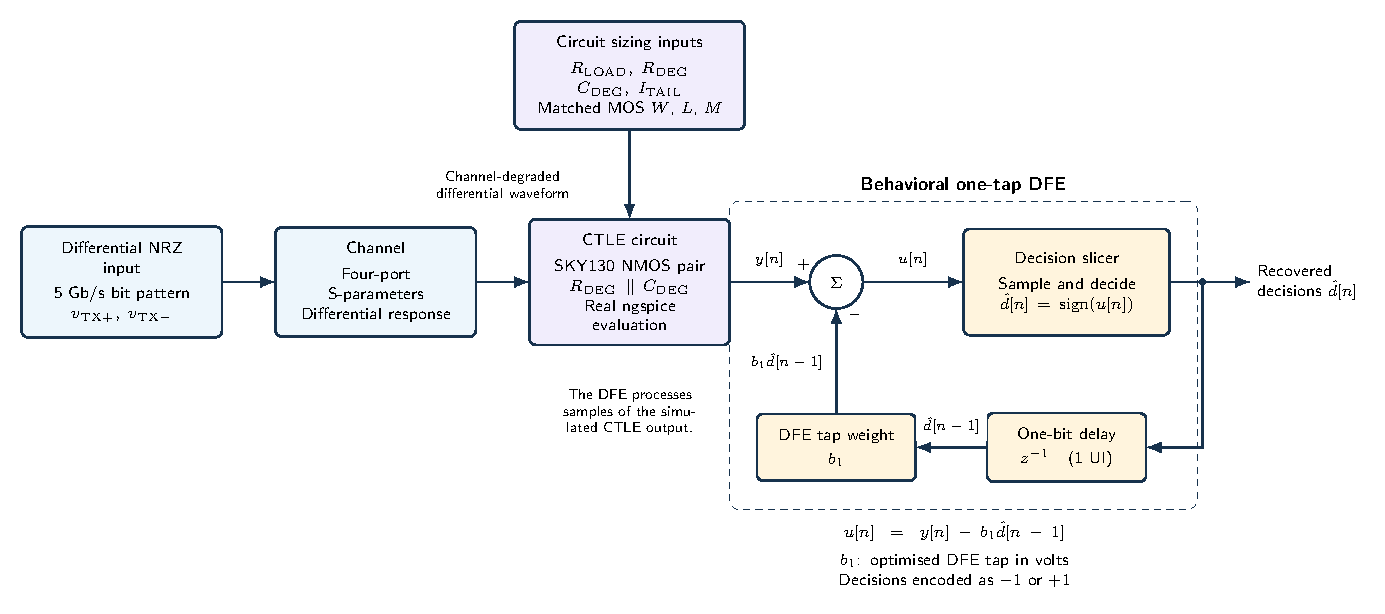
\includegraphics[width=\textwidth]{receiver-signal-path.pdf}
  \caption{Implemented receiver signal path. A differential \SI{5}{Gb/s} NRZ
  stimulus is filtered by a four-port channel and applied to the
  transistor-level SKY130 CTLE. The one-tap DFE operates on sampled CTLE output
  values in software. Its feedback subtracts the previous decision, weighted by
  the optimized tap $b_1$, before the current decision is made. The dashed DFE
  boundary is behavioral and must not be interpreted as a transistor schematic.}
  \label{fig:signal-path}
\end{figure}

As shown in \cref{fig:signal-path}, the electrical and behavioral portions have
different validation strength. The CTLE waveform comes from ngspice. Channel
filtering and DFE processing are numerical models. The recovered decisions are
therefore appropriate for design-space exploration but do not include sampler
noise, comparator offset, metastability, feedback delay, or clock jitter.

\section{Software layers}

\begin{description}
  \item[Simulation layer.] \code{simulator/} renders benches, launches ngspice,
  parses outputs, validates S-parameters, filters waveforms, and calculates
  receiver metrics.
  \item[Optimization layer.] \code{rl/} defines parameter grids, state and
  reward schemas, PPO models, checkpoints, and the environment contract.
  \item[Experiment layer.] \code{experiments/} supplies training, evaluation,
  search, qualification, and web-interface entry points.
  \item[Analysis layer.] \code{analysis/} builds specification tables,
  comparisons, qualification summaries, plots, and design catalogs.
\end{description}

The primary receiver API is \code{simulator.receiver.evaluate\_receiver()}.
It returns success status, the first failed stage, combined metrics, per-stage
records, warnings, provenance, runtime, and cache identity.

\section{Traceability and failure handling}

Every expensive evaluation is associated with the circuit parameters,
conditions, channel and port map, model files, ngspice identity, metric schema,
and implementation fingerprints. Hard failures stop later work; execution
failures remain distinguishable from deterministic constraint failures. This is
important because a missing measurement must never be interpreted as a passing
value.

\section{Dashboard and generated deliverables}

The local web interface is a thin controller over the same command-line pipeline
rather than a second evaluator. It provides structured numeric target fields,
backend and PPO-version selection, checkpoint discovery, channel and port-map
configuration, PVT scope, and optional final HD3/noise and eye generation. It
launches each run in a subprocess so a simulator or numerical failure does not
silently corrupt the server state.

Recorded events can be transformed into a bounded SVG run graph whose nodes
represent configuration, targets, checkpoints, candidates, simulator stages,
cache origins, failures, selection, qualification conditions, and artifacts.
The browser view is intentionally abbreviated for large runs; downloadable JSON
retains the complete record. Per-run plots cover reward, strict success, losses,
entropy, electrical metrics, failure stages, and evaluation latency. Missing
measurements appear as gaps rather than zero-valued points.

For a successfully selected design, the output set can include the final
parameter vector, strict specification verdicts, raw JSON and JSONL records,
run-graph JSON/SVG, a parameterized SPICE netlist, a schematic representation,
and CTLE/behavioral-DFE eye artifacts. These outputs are the appropriate judging
interface because they connect a visible result to machine-readable evidence.

\chapter{Receiver and Channel Models}

\section{Continuous-time linear equalizer}

The CTLE is a matched NMOS differential pair with resistive loads, parallel
source-degeneration resistance and capacitance, and an ideal tail-current
source. Its tunable quantities are $R_{\mathrm{LOAD}}$, $R_{\mathrm{DEG}}$,
$C_{\mathrm{DEG}}$, $I_{\mathrm{TAIL}}$, and, in the expanded v3 schema, MOS
width, length, and multiplier. The differential circuit is electrically
inverting, so the benches define the logical output polarity consistently.

At low frequency, $C_{\mathrm{DEG}}$ is approximately open and
$R_{\mathrm{DEG}}$ reduces effective transconductance. At increasing frequency,
the capacitor bypasses part of the degeneration and raises the effective gain.
The zero is approximately
\begin{equation}
  f_z \approx \frac{1}{2\pi R_{\mathrm{DEG}}C_{\mathrm{DEG}}}.
\end{equation}
The complete response also depends on transistor transconductance, output
resistance, load resistance, parasitic capacitance, and the operating point.
Consequently, this expression explains the tuning direction but does not replace
the simulated transfer function.

The current Stage~1 model uses ideal resistors, capacitors, and a tail-current
source. Its computed MOS channel area is only a partial geometry measure; no
total receiver area is claimed.

\section{Four-port channel}

\code{simulator/channel.py} parses Touchstone 1.x four-port data, supports
RI, magnitude-angle, and dB-angle formats, and constructs the differential
transfer $S_{dd21}$. Before transient filtering, the channel is checked for port
mapping, monotonic frequency data, reference impedance, bandwidth, passivity,
and causal behavior. The public development channel and the included synthetic
regression channel are useful test inputs, but neither constitutes PCI-SIG
compliance evidence.

\section{Behavioral one-tap DFE}

For sampled CTLE output $y[n]$, tap $b_1$, and previous decision
$\hat d[n-1]\in\{-1,+1\}$, the DFE uses
\begin{equation}
  u[n] = y[n] - b_1\hat d[n-1], \qquad
  \hat d[n] = \operatorname{sign}(u[n]).
\end{equation}
The implementation first trains or selects a sampling phase, then evaluates
locked-phase eye height, contiguous eye width, decision margin, and observed
errors. Percentile-based vertical metrics reduce sensitivity to single-sample
outliers. The model does not simulate the physical feedback amplifier, slicer,
clock path, or adaptation circuitry.

\chapter{Simulation and Evaluation Methodology}

The evaluator is hierarchical: inexpensive checks reject invalid candidates
before costly transient and qualification work. \Cref{fig:optimization-flow}
shows the complete search and verification boundary.

\begin{figure}[p]
  \centering
  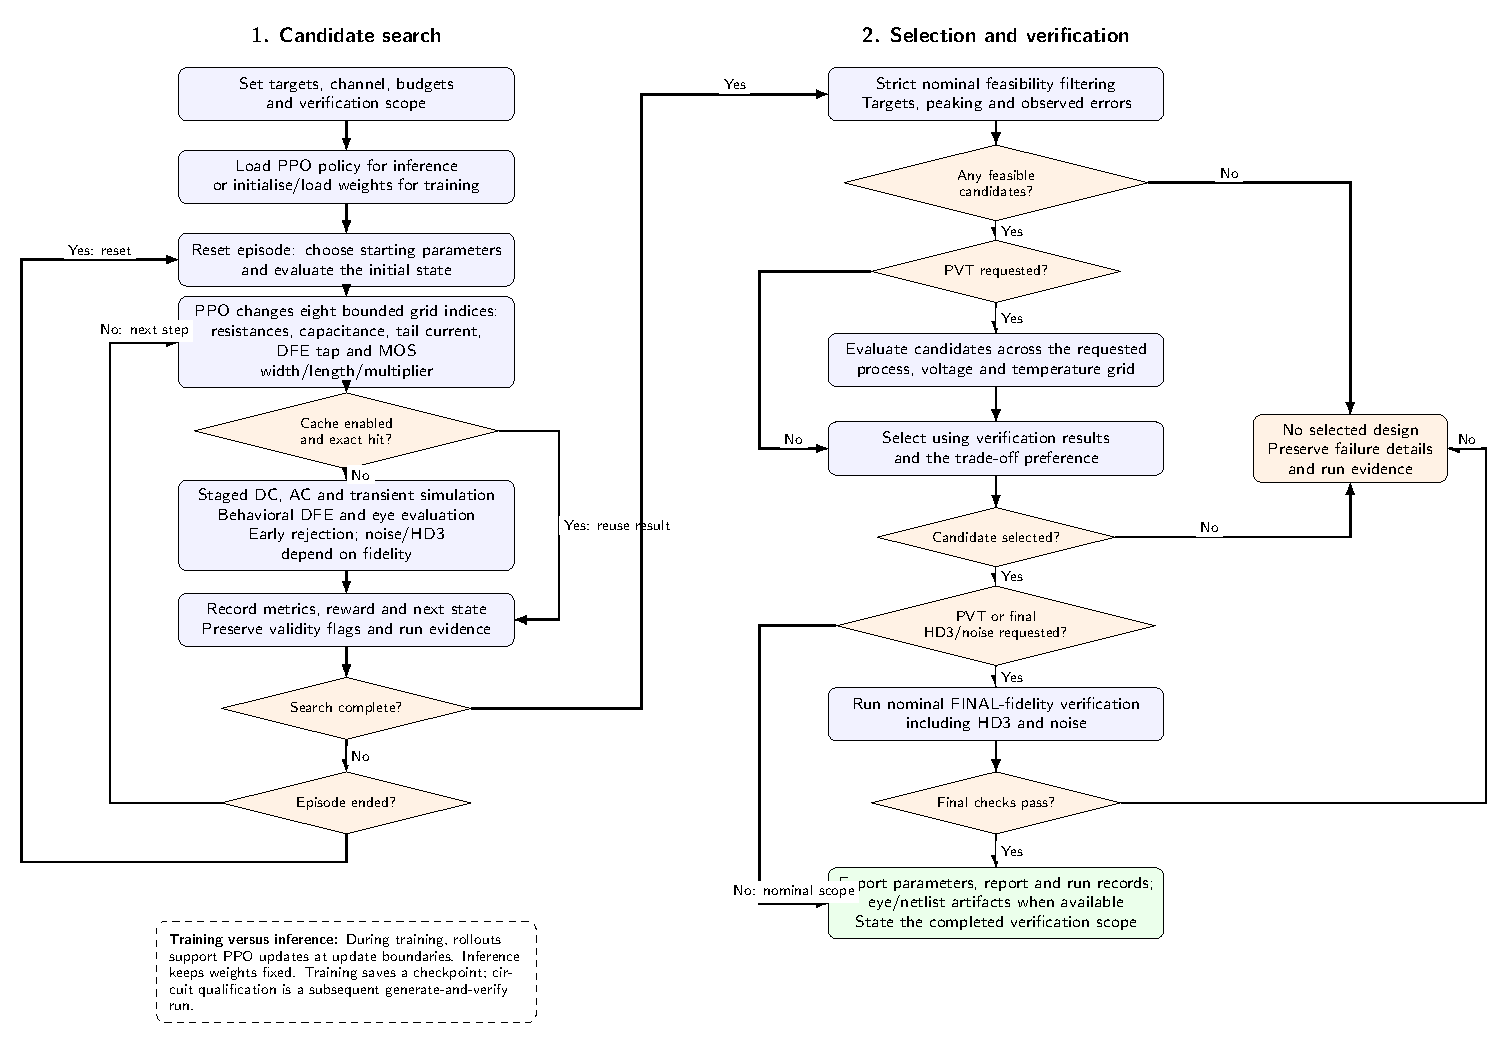
\includegraphics[width=\textwidth,height=0.82\textheight,keepaspectratio]{optimization-flow.pdf}
  \caption{Candidate search, selection, and verification flow. PPO changes
  bounded parameter-grid indices and receives metrics from the common staged
  evaluator. Exact cache hits reuse deterministic results. Candidate generation
  is followed by strict nominal filtering; optional PVT and final-fidelity
  checks occur only after a feasible design exists. Training saves a policy,
  while inference keeps policy weights fixed.}
  \label{fig:optimization-flow}
\end{figure}

\section{Evaluation stages}

\begin{table}[htbp]
\centering
\caption{Principal stages of a receiver evaluation.}
\label{tab:stages}
\begin{tabularx}{\textwidth}{@{}l X X@{}}
\toprule
Stage & Purpose & Representative outputs \\
\midrule
Validation & Check parameters, files, models, and conditions & Structured setup failure \\
DC & Establish bias, balance, common mode, and headroom & CTLE power and operating point \\
AC & Characterize differential transfer & Peaking, peak frequency, group delay \\
CTLE transient & Reject gross swing or rail violations & Input/output swing \\
Channel & Validate and characterize the S4P network & Loss, delay, passivity, causality \\
Noise & Integrate input-referred noise & RMS noise from \SI{10}{MHz}--\SI{5}{GHz} \\
HD3 & Fit the harmonic content of a sine response & Third-to-fundamental ratio \\
Receiver transient & Evaluate the channel-driven CTLE and DFE & Eye, margin, errors, transient power \\
\bottomrule
\end{tabularx}
\end{table}

\section{Fidelity levels}

Screening runs DC, AC, and a short channel-free diagnostic. Training adds the
channel and a 128-bit receiver evaluation. Candidate fidelity uses 512 bits and
enables noise and one-amplitude HD3. Final fidelity uses a 1024-bit request and
additional HD3 amplitudes. The number of useful post-warm-up bits can be smaller
than the requested sequence; result tables should therefore report the recorded
\code{simulated\_bits} value rather than infer it from the fidelity name.

\section{Caching and provenance}

The content-addressed cache is valid only when the complete evaluation identity
matches. The identity includes design parameters, environment conditions,
channel checksum and port map, model and bench checksums, schema versions, and
simulator configuration. Retryable execution failures are not treated as valid
cached circuit results.

\chapter{PPO Formulation and Version Evolution}

Nebula's PPO subsystem evolved through three versioned formulations with
explicit compatibility checks, so changes to the state, reward, and design space
could be evaluated without silently changing historical checkpoints. All versions use separate two-layer, 64-unit tanh policy
and value networks, generalized advantage estimation with $\gamma=0.99$ and
$\lambda=0.95$, PPO clipping $\epsilon=0.2$, and entropy coefficient 0.01
\citep{schulman2017ppo,schulman2016gae}. Each parameter has an independent
categorical action head whose default choices map to grid-index deltas
$\{-1,0,+2\}$, clipped at the grid boundaries.

\section{PPO v1: AutoCkt-style baseline}

PPO v1 established the first end-to-end RL-to-SPICE path. Its five variables are
$R_{\mathrm{LOAD}}$, $R_{\mathrm{DEG}}$, $C_{\mathrm{DEG}}$,
$I_{\mathrm{TAIL}}$, and the behavioral DFE tap. Each uses a 21-point grid. An
action updates parameter index $i$ according to
\begin{equation}
  k_{i,t+1}=\operatorname{clip}\!\left(k_{i,t}+\Delta_{i,t},0,N_i-1\right),
  \qquad \Delta_{i,t}\in\{-1,0,+2\}.
\end{equation}

The 13-dimensional state contains four signed relative errors between achieved
and requested targets, four target-to-reference descriptors, and five normalized
parameter indices. The target metrics are locked-phase DFE eye height, DFE eye
width, DFE decision margin, and CTLE power.

The reward follows the AutoCkt-style rule \citep{wang2020autockt}: only
unsatisfied relative errors contribute negative values, and a design within the
terminal tolerance receives 10. Nebula adds an explicit $-1$ result for simulator
failure instead of allowing absent output to crash the environment.

V1 proved that PPO actions could drive parameterized SPICE evaluations, but it
exposed two information problems. Reset built an observation from zero-filled
metrics rather than evaluating the starting circuit. In addition, all early
failures received the same $-1$ reward. In the fair no-warm-start real-SPICE
comparison, all 20 PPO trials failed at DC and produced identical reward, leaving
no signal to distinguish their actions.

\section{PPO v2: valid observations and informative failures}

PPO v2 was developed as an additive correction while retaining v1 state, reward,
action, and checkpoint behavior for reproducibility.

First, optional \emph{evaluated reset} simulates the initial circuit so the first
observation represents a genuine result. It costs one evaluation per episode but
removes the artificial-zero state. Second, the 28-dimensional v2 state retains
the 13 v1 entries and adds one validity flag, early-stage CTLE-power and
AC-peaking information, and a 12-way one-hot failure-stage code. The policy can
therefore distinguish setup, DC, AC, channel, and transient outcomes. Missing
receiver metrics are never silently interpreted as measured zeros.

Third, structured reward v2 gives an uninformative early failure a structural
floor of $-20$, below every valid graded design. Where genuine measurements
exist, individual target components and early-stage margins provide distance
information. A strict pass receives the terminal bonus plus a bounded overshoot
bonus capped at 2. The result separately records the legacy tolerance-based
terminal criterion and the exact strict target verdict.

V2 also added safe full checkpoints containing policy/value weights, optimizer
state, Python/NumPy/PyTorch RNG states, counters, hyperparameters, grids, target
IDs, schema versions, and Git identity. Incompatible schemas are rejected before
weights are loaded. Versioned step/update events record actions, boundary
clipping, metrics, failures, rewards, losses, entropy, and evaluation count.

The changes were tested in a 20-seed synthetic ablation from an infeasible
corner. Strict satisfaction was 0/20 for every variant at the small budget, so
the experiment does not prove circuit improvement. Under a uniform looser
criterion, corrected reset did not regress relative to v1 (3 wins, 17 ties), the
validity-aware state beat v1 in 13/20 seeds, and the full reward-v2 stack beat v1
in 15/20 seeds. Symmetric $\{-1,0,+1\}$ actions were worse in all 20 seeds and
were rejected. These are synthetic software-landscape results; no large
real-SPICE PPO v2 study was completed.

\section{PPO v3: expanded sizing and runtime contract}

PPO v3 builds on v2's failure semantics while expanding the design space from
five to eight variables. It adds matched MOS width $W$, length $L$, and integer
multiplier $M$. Both input transistors always share geometry, preserving the
matched-pair invariant. V3 has eight categorical action heads and retains the
$\{-1,0,+2\}$ grid deltas. The multiplier remains integer-valued through action
decoding, serialization, and SPICE rendering.

The frozen v3 state has 52 components: target errors and references; eight
normalized indices; diagnostic values and their validity flags; evaluator-stage
identity; channel loss at \SIlist{1.25;2.5;5}{GHz} and bulk delay; partial MOS
channel-area context; and an explicit false total-area-valid flag. Channel
features prevent evaluation on a new channel from appearing identical to the
training environment.

Reward v3 begins with reward v2 and tightens termination. Success requires a
successful evaluation, all four targets, peaking inside \SIrange{3}{12}{dB}, and
zero observed DFE errors. A weight-0.02 regularizer favors smaller matched-MOS
channel area when available. It cannot override feasibility and cannot establish
the competition's total-area requirement.

V3 checkpoints bind the policy to the ordered eight-parameter registry, exact
grids, channel checksum and port map, backend, fidelity, toolchain, and schema
versions. A five-head v1/v2 checkpoint cannot load as v3. The registry is shared
with Random Search, CEM, PVT, schematic export, and the UI.

The preserved v3 summary records a completed real-backend run with seed 101,
100 updates, and 692 evaluations. This demonstrates expanded-agent integration
with real SPICE. It does not prove v3 superior to v2, arbitrary-start convergence,
or near-optimality.

\section{Version comparison}

\begin{table}[htbp]
\centering
\caption{Technical evolution of PPO in Nebula.}
\label{tab:ppo-versions}
\begin{tabularx}{\textwidth}{@{}l c c X X@{}}
\toprule
Version & State & Heads & Main development & Evidence boundary \\
\midrule
v1 & 13 & 5 & First AutoCkt-style RL-to-SPICE baseline & End-to-end operation; flat early-failure reward exposed \\
v2 & 28 & 5 & Evaluated reset, validity/failure state, structured reward, resumable checkpoints & Multi-seed synthetic ablation; no large real-SPICE v2 proof \\
v3 & 52 & 8 & MOS $W/L/M$, channel context, stricter termination, partial-area regularizer & Real-backend artifact; no proven v2/v3 superiority \\
\bottomrule
\end{tabularx}
\end{table}

The progression is best understood as closure of the automation contract: v1
connected PPO to SPICE, v2 repaired information quality and reproducibility, and
v3 expanded physical sizing and bound downstream tools to a common identity.

\section{Random Search and CEM}

Random Search draws independent bounded candidates. CEM updates a distribution
toward an elite subset. Both use the same target and receiver evaluator as PPO.
A fair comparison must control evaluation count, time, seed, initialization,
target, channel, fidelity, and success definition. PPO is sequential and
grid-local, whereas the baselines can make global continuous draws; that
structural difference must accompany any short-horizon result.

\chapter{Experimental Setup}

The report separates nominal evaluation, historical PVT qualification, and
optimizer comparison. Numbers from different candidates or runs are not merged.

\section{Recorded v3 training run}

The preserved \code{results/v3\_tt\_1000\_summary.json} records a real-backend
v3 run with seed 101, 100 policy updates, and 692 evaluations. Its best recorded
reward was 10.3096. This artifact establishes that a real-SPICE training run
completed and produced a checkpoint; it does not by itself prove global
convergence or optimizer superiority.

\section{Completed reduced 27-condition qualification}

The primary artifact is
\code{results/web\_ui\_runs/07acbcab1cd346cca24eab31919496c0.json}.
It evaluates selected design \code{pipeline\_ep0} over TT, SS, and FF; three
supply values; and temperatures of 0, 27, and \SI{125}{\degreeCelsius}. All 27
conditions passed at candidate fidelity using a 512-bit request; every condition
records 425 useful simulated bits after alignment and warm-up. The channel is
\code{ieee802\_ibm\_20db\_thru.s4p}, checksum
\code{ce6002f8663623eb...}, with port map 1,3,2,4. This is a completed reduced
grid, not the full five-corner competition matrix.

\section{Fair optimizer comparison}

The no-warm-start comparison gives each method 20 evaluations with seed 123 and
the same success criterion. Random Search samples globally in the continuous
space; CEM uses a centered Gaussian; PPO begins at the parameter-grid midpoint
and uses horizon-one local actions. The budget is matched, but these action-space
differences remain.

\section{Experimental identity}

For any new run, the following fields should accompany the reported result:
repository revision and dirty status; Python, ngspice, and model versions;
design identifier and full parameters; target; channel checksum and port map;
seed and budget; fidelity; PVT set; and result-artifact checksum. Appendix
\ref{app:reproducibility} gives the corresponding commands.

\section{Verification strategy}

The automated suite covers parameter parsing and bounds, netlist rendering,
ngspice process/error handling, channel validation, receiver metrics, PPO
state/action/reward schemas, checkpoint compatibility, event emission, caching,
baseline wiring, PVT selection, specification generation, schematic export, run
graphs, and web-command construction. Optional integration tests exercise
ngspice and SKY130 only when external dependencies are configured.

Passing tests establish software behavior for the tested cases; they do not
establish analog performance over unsampled parameters or conditions. The final
submission should include a dated log from a clean commit and separately report
unit, simulator-integration, and skipped tests.

The most useful end-to-end invariants are that all eight v3 parameters reach
every relevant bench and artifact; cache identity changes with every electrical
input; missing metrics stay missing; incompatible checkpoints fail before
simulation; and nominal success is never promoted to PVT success.

\chapter{Results}

\section{Selected design and evaluation contract}

The primary result in this report is run
\code{07acbcab1cd346cca24eab31919496c0}, which selected
\code{pipeline\_ep0} using the PVT rank ``most robust.'' The target was
locked-phase DFE eye height $>\SI{0.1}{V}$, eye width $>0.4$ UI, decision
margin $>\SI{0}{V}$, and CTLE power $<\SI{15}{mW}$. The run used PPO v3
checkpoint \code{ppo\_v3\_tt\_1000\_policy.pt}, the IEEE/IBM 20-dB-through
development channel, port map 1,3,2,4, and candidate-fidelity PVT evaluation.

\begin{table}[htbp]
\centering
\caption{Eight parameters of the selected design used in the completed
27-condition run.}
\label{tab:selected-design}
\begin{tabular}{@{}l r l@{}}
\toprule
Parameter & Value & Unit \\
\midrule
$R_{\mathrm{LOAD}}$ & 2457.143 & $\Omega$ \\
$R_{\mathrm{DEG}}$ & 485.714 & $\Omega$ \\
$C_{\mathrm{DEG}}$ & 0.485714 & pF \\
$I_{\mathrm{TAIL}}$ & 0.670 & mA \\
Behavioral DFE tap & 57.143 & mV \\
Matched MOS width $W$ & 10.378 & $\mu$m \\
Matched MOS length $L$ & 0.150 & $\mu$m \\
MOS multiplier $M$ & 1 & integer \\
\bottomrule
\end{tabular}
\end{table}

The channel checksum is
\path{ce6002f8663623ebc0992c458c3d518faf79ccfeb65d1ee59c8c638bccd66581}.
The PVT request contains 512 bits; each corner records 425 useful simulated bits
after alignment and warm-up. These identifiers are necessary because results
from other candidates and channels are not interchangeable.

\section{Completed reduced 27-condition PVT run}

All 27 evaluated conditions passed over TT/SS/FF,
\SIlist{1.71;1.80;1.89}{V}, and \SIlist{0;27;125}{\degreeCelsius}.
\Cref{fig:pvt-heatmaps} displays the recorded values for every condition.

\begin{landscape}
\begin{figure}[p]
  \centering
  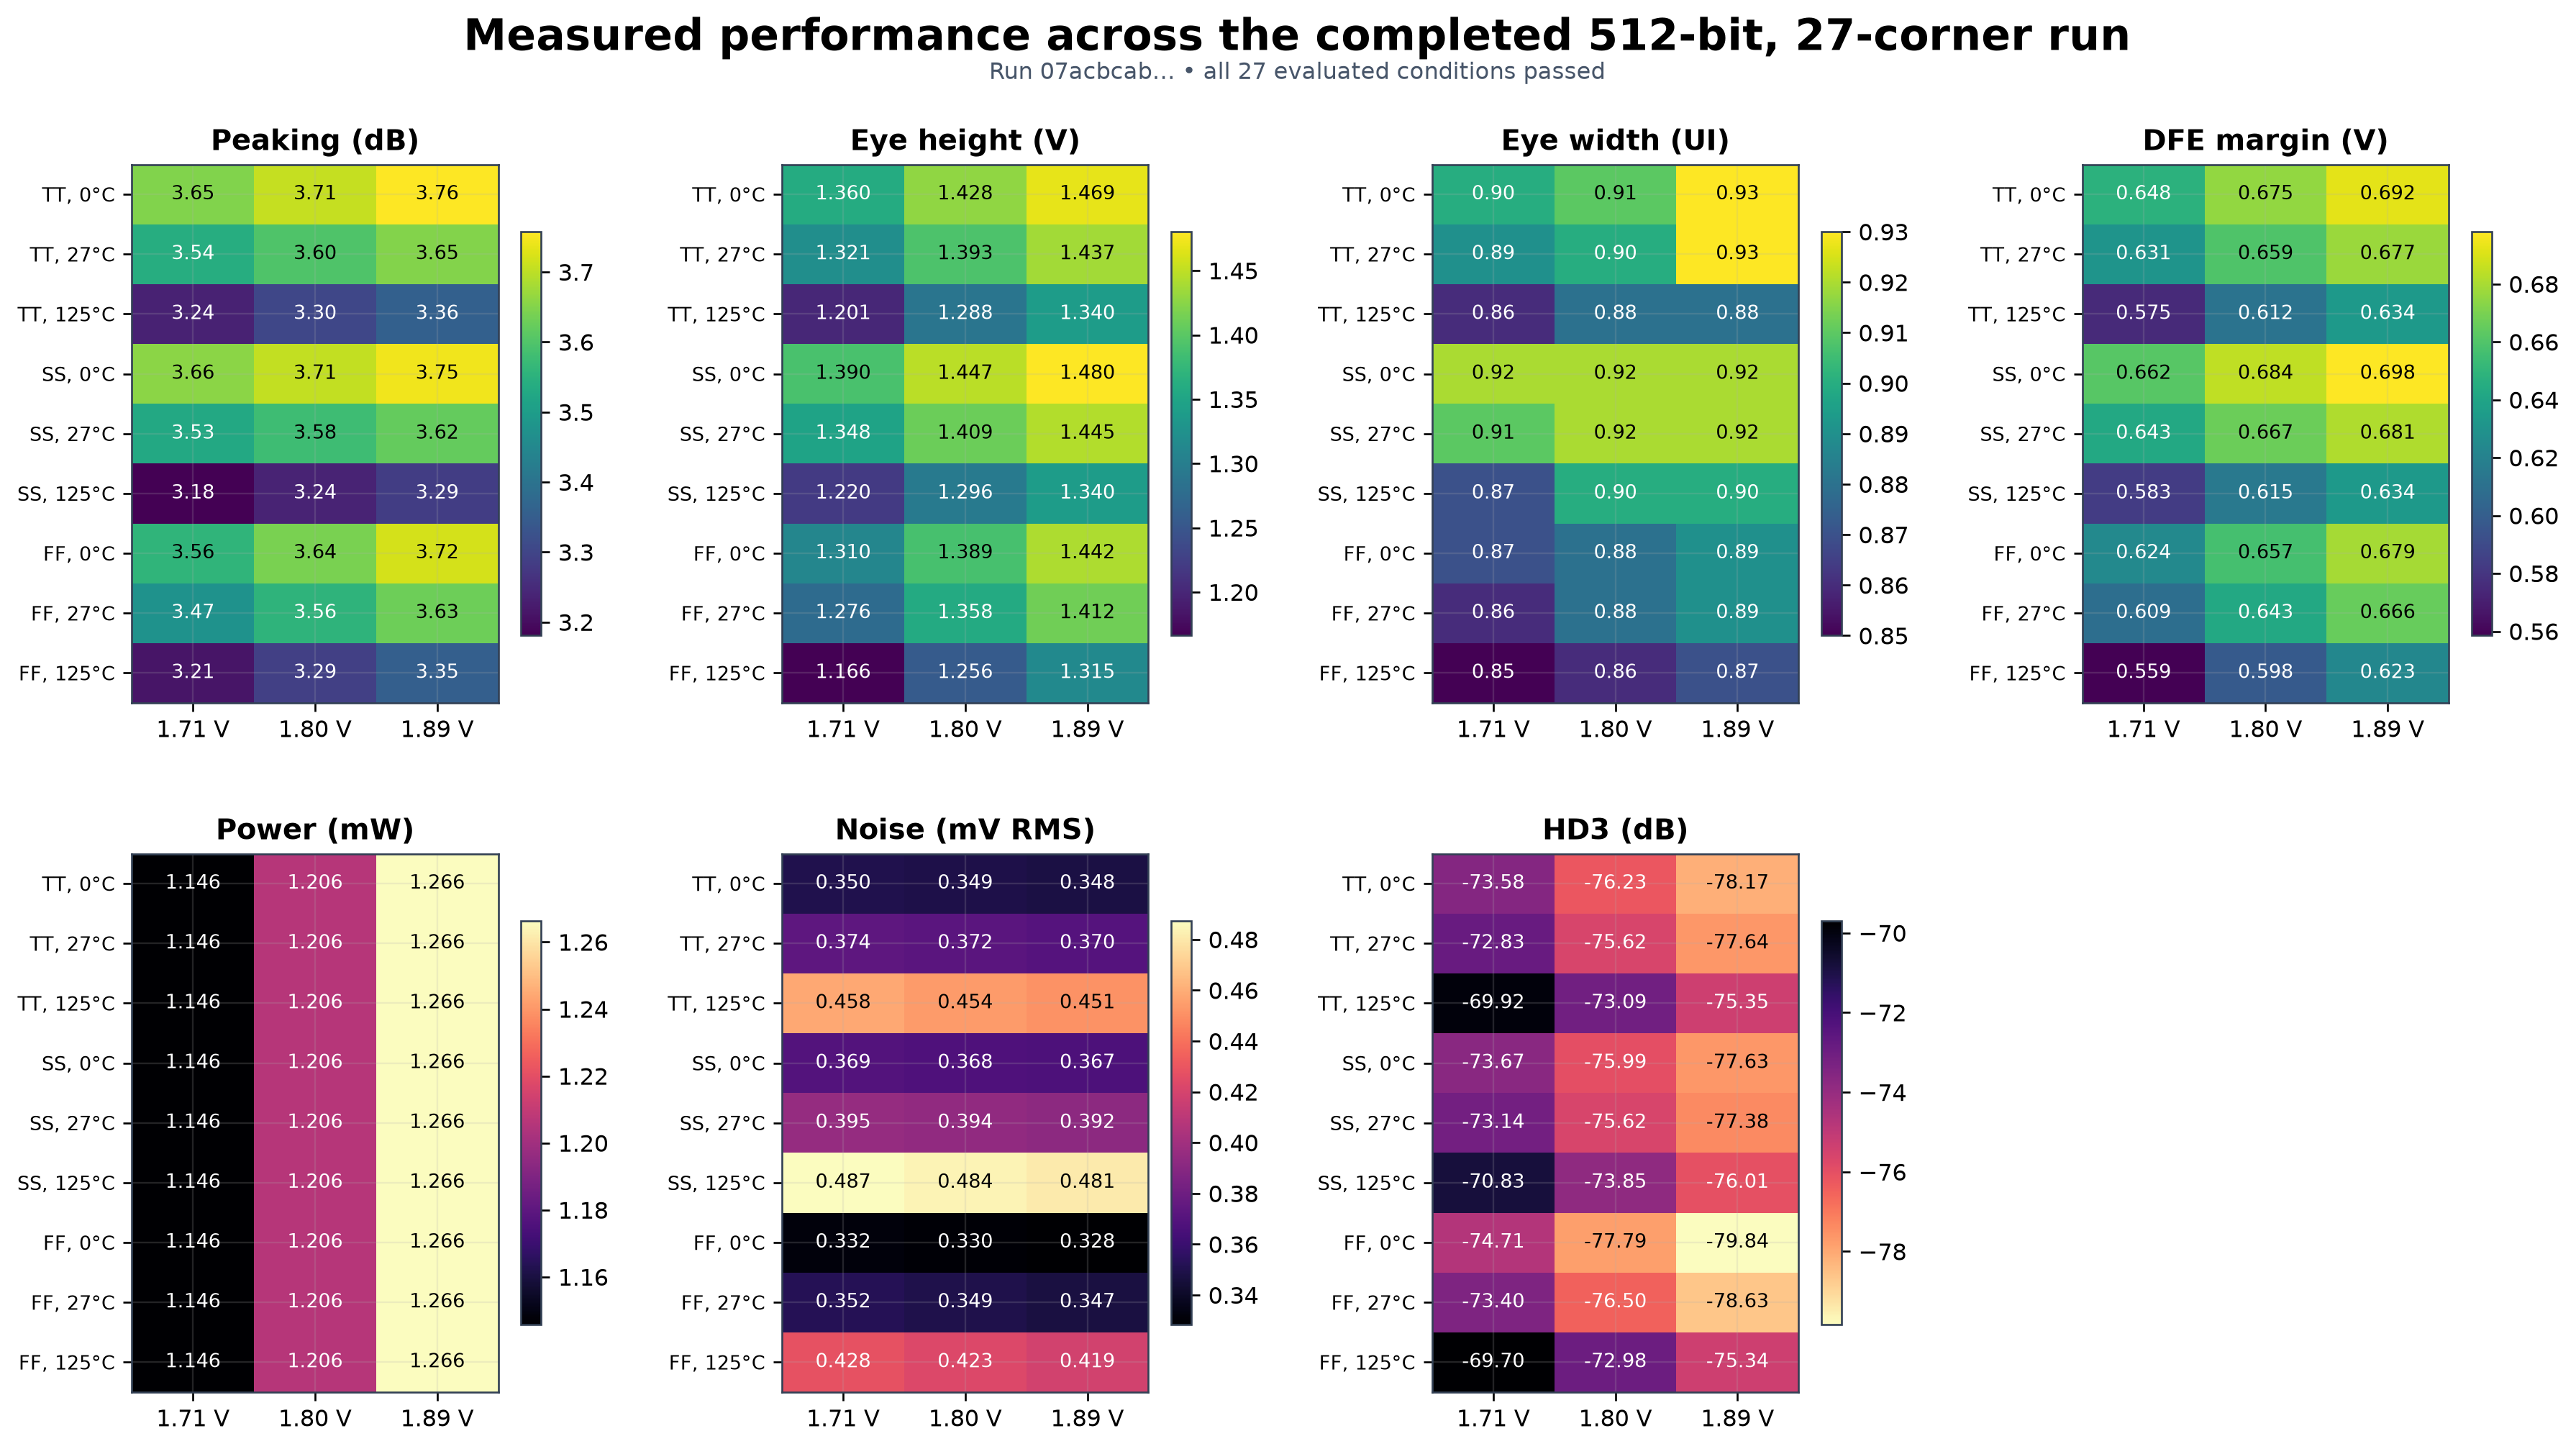
\includegraphics[width=0.98\linewidth]{pvt27-all-metrics-heatmaps.png}
  \caption{Measured performance across the completed 512-bit, 27-condition
  candidate-fidelity run. All values come from run \code{07acbcab...}; all 27
  conditions passed. Power is CTLE power. The DFE metrics are behavioral, and
  zero finite-pattern errors are not a BER result. This reduced grid excludes
  \SI{75}{\degreeCelsius}, SF, and FS.}
  \label{fig:pvt-heatmaps}
\end{figure}
\end{landscape}

\begin{figure}[htbp]
  \centering
  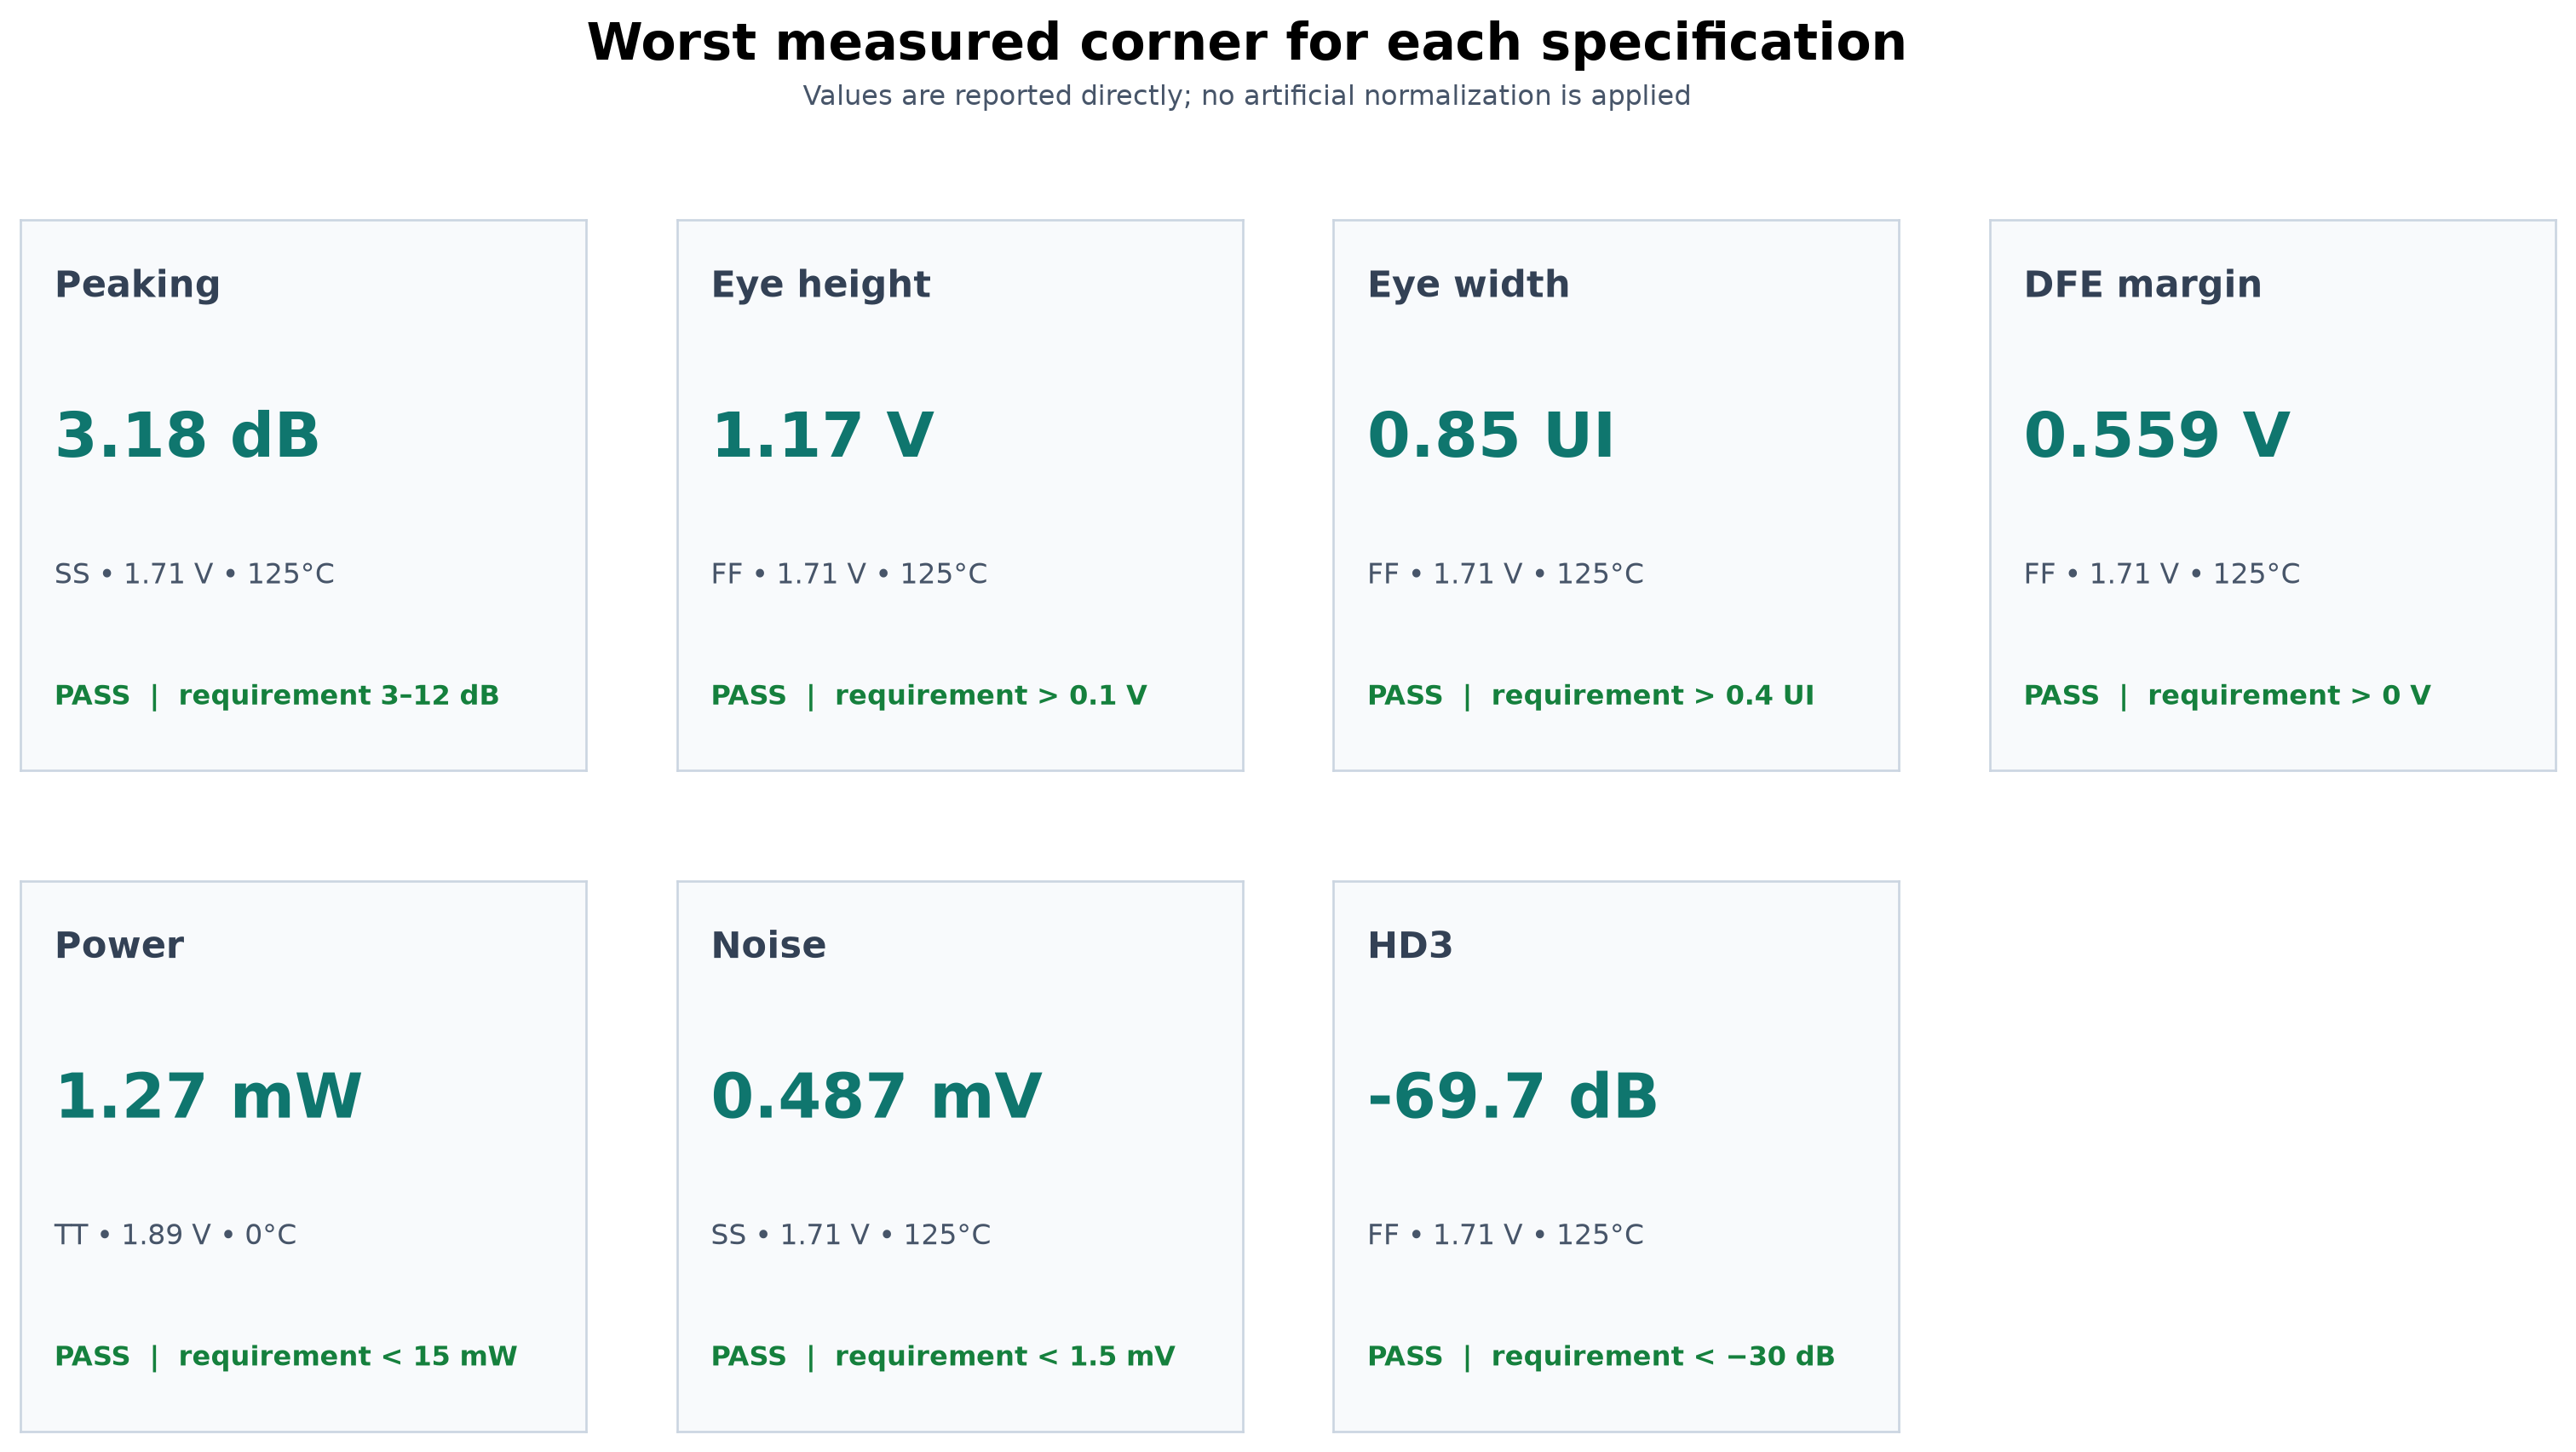
\includegraphics[width=0.96\textwidth]{pvt27-worst-case-spec-margins.png}
  \caption{Worst recorded corner for each evaluated specification in run
  \code{07acbcab...}. The plot reports measured values and locations directly;
  it does not normalize the margins into an aggregate score.}
  \label{fig:pvt-worst}
\end{figure}

The worst locked-phase eye height was \SI{1.16620}{V} at FF,
\SI{1.71}{V}, \SI{125}{\degreeCelsius}; worst eye width was 0.85 UI at the
same corner; and worst DFE margin was \SI{0.55852}{V}. CTLE power ranged from
\SI{1.1457}{mW} to \SI{1.2663}{mW}. Input-referred noise ranged from
\SI{0.328262}{mV RMS} to \SI{0.487290}{mV RMS}. The least favorable HD3
(largest value) was \SI{-69.6987}{dB} at FF, \SI{1.71}{V},
\SI{125}{\degreeCelsius}. Peaking remained between 3.18078 and
\SI{3.75745}{dB}.

These margins demonstrate robust behavior over the reduced grid, but not the
unmeasured competition corners or physical implementation effects.

\section{CTLE AC response}

\begin{landscape}
\begin{figure}[p]
  \centering
  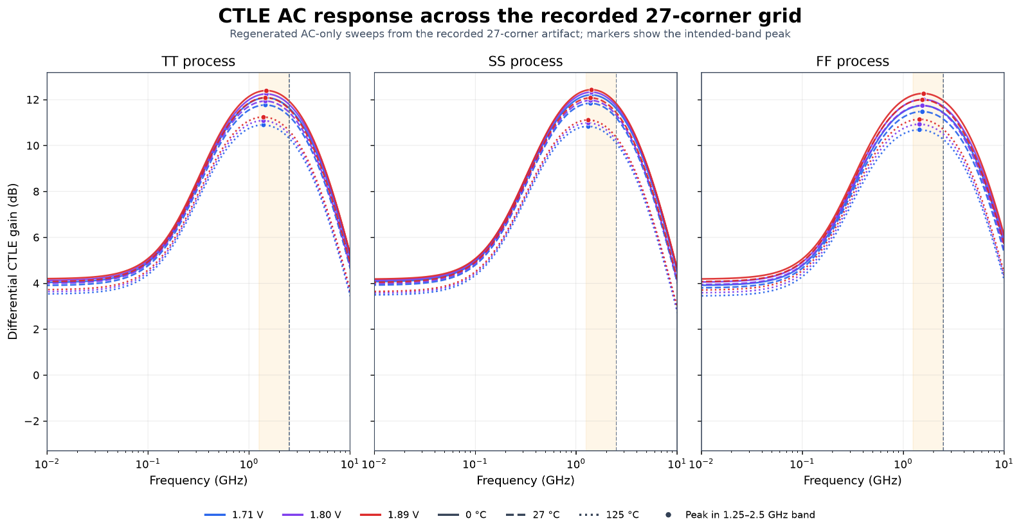
\includegraphics[width=0.96\linewidth]{ctle-ac-responses-27-corners.png}
  \caption{Regenerated AC-only ngspice sweeps for the selected design and the 27
  recorded process/voltage/temperature conditions. The shaded region marks the
  intended \SIrange{1.25}{2.5}{GHz} peak band and the dashed line marks the
  \SI{2.5}{GHz} Nyquist frequency. These curves were regenerated from the run
  configuration; they are not stored transient/noise/HD3 waveforms and do not by
  themselves prove PVT qualification.}
  \label{fig:ac-corners}
\end{figure}
\end{landscape}

\section{PPO v3 training evidence}

The recorded seed-101 v3 training run completed 100 updates and 692 real-backend
evaluations. \Cref{fig:ppo-training} shows reward, cumulative satisfying steps,
and the first failed stage. The dominant AC failures explain why staged
diagnostics and validity-aware state are important. The curve is one training
history, not a confidence interval or proof of convergence.

\begin{landscape}
\begin{figure}[p]
  \centering
  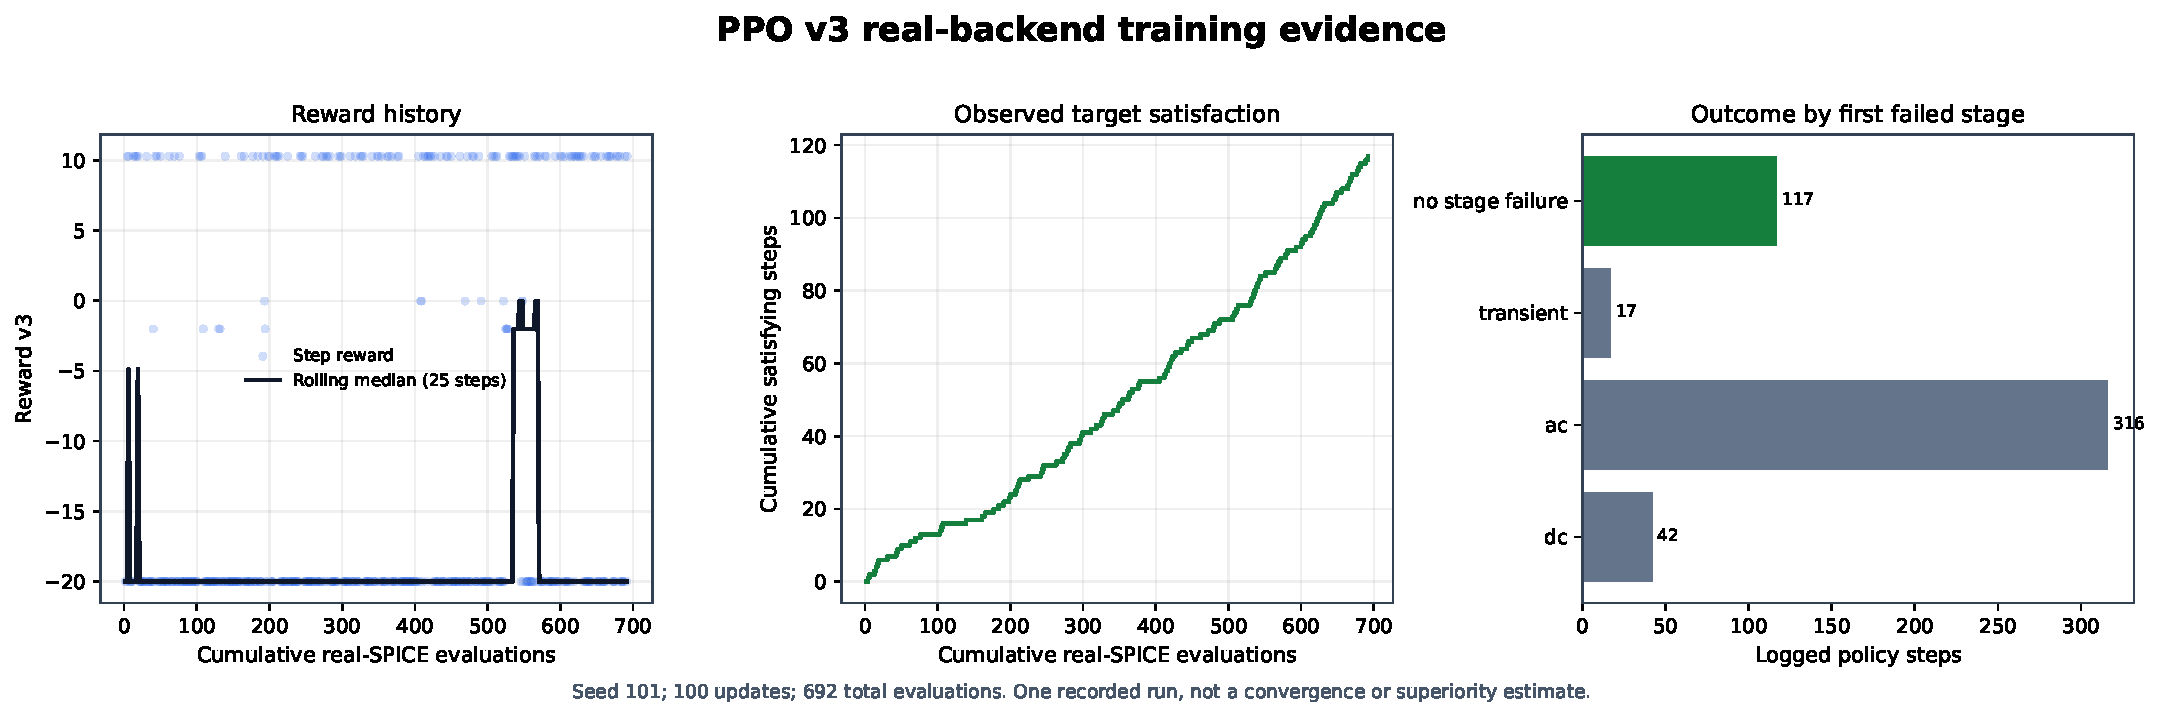
\includegraphics[width=0.97\linewidth]{ppo-v3-training-overview.pdf}
  \caption{PPO v3 real-backend training evidence from
  \code{v3\_tt\_1000\_training.jsonl}. Reward v3 values must not be compared
  directly with v1/v2 reward scales. Cumulative satisfying steps are within-run
  observations, not independent trials.}
  \label{fig:ppo-training}
\end{figure}
\end{landscape}

\section{Fair optimizer comparison}

\begin{figure}[htbp]
  \centering
  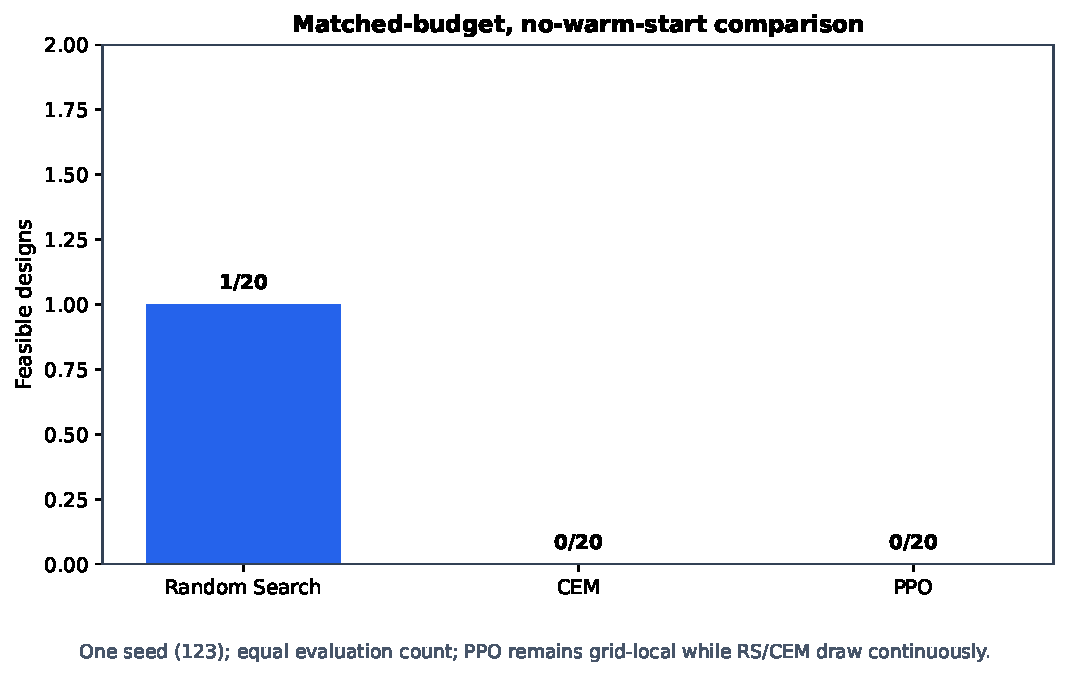
\includegraphics[width=0.78\textwidth]{optimizer-comparison.pdf}
  \caption{The matched-budget, no-warm-start comparison used one seed and 20
  evaluations per method. Random Search found one feasible design; CEM and PPO
  found none. PPO was grid-local while the baselines used continuous draws, so
  the experiment is insufficient for a general optimizer ranking.}
  \label{fig:optimizer-comparison}
\end{figure}

PPO superiority is not demonstrated. The result instead reveals a practical
reachability limitation under the tested short-horizon configuration.

\section{Evaluation efficiency}

Hierarchical early rejection avoids later stages after a hard failure, while
exact-key caching avoids repeated identical evaluations. In a controlled
20-seed synthetic study, caching reduced evaluator calls from 1200 to 1085
(9.58\%) with bit-identical action and reward trajectories. Synthetic wall-clock
time fell by only 1.41\% because PPO computation dominated the cheap algebraic
evaluator. A matched real-SPICE cache timing experiment and an exhaustive
MOS/R/C/L baseline were not completed; therefore significant real design-time
speedup and near-optimality remain unproven.

\section{Recorded eye artifact}

\IfFileExists{../results/v3_tt_1000_eye.png}{%
\begin{figure}[htbp]
  \centering
  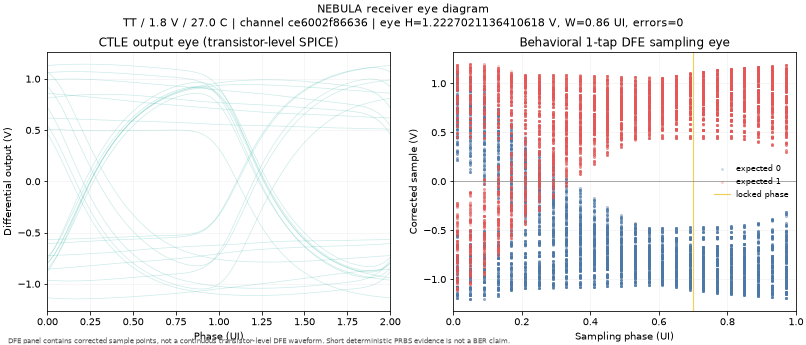
\includegraphics[width=\textwidth]{v3_tt_1000_eye.png}
  \caption{Repository-backed eye artifact. The left panel is the continuous
  transistor-level CTLE output after channel filtering; the right panel contains
  corrected sample points from the behavioral one-tap DFE. The DFE panel is not
  a transistor-level waveform, and the finite pattern is not BER evidence.}
  \label{fig:eye}
\end{figure}
}{\emph{The optional eye artifact was not found when this document was built.}}

\section{Result boundary}

The evidence establishes a working, versioned automation pipeline with real
ngspice in the loop, a completed reduced-grid PVT run, and preserved experiment
artifacts. It does not establish a complete physical receiver, general PPO
superiority, full five-corner PVT, PCIe compliance, total area, or near-optimality.

\chapter{Using the Code}

The repository is available at \href{\projecturl}{\projecturl}. Python 3.10 or
newer, NumPy, ngspice, and a compatible SKY130A ngspice model library are
required for real-circuit evaluation. Commands below assume the repository root
as the working directory.

\section{Create an environment}

\begin{lstlisting}[language=bash]
python -m venv .venv
# Windows PowerShell
.\.venv\Scripts\Activate.ps1
python -m pip install -r requirements.txt
\end{lstlisting}

Set the external tools without committing machine-specific paths:

\begin{lstlisting}[language=bash]
$env:NGSPICE_EXECUTABLE = "C:\path\to\ngspice_con.exe"
$env:SKY130_MODEL_LIBRARY = "C:\path\to\sky130.lib.spice"
\end{lstlisting}

\section{Run the regression suite}

\begin{lstlisting}[language=bash]
python -m unittest discover -v
\end{lstlisting}

Tests requiring the SKY130 model are skipped when the model variable is not
configured. The exact executed, passed, failed, and skipped counts should be
recorded together with the date, commit, and interpreter.

\section{Evaluate one receiver design}

\begin{lstlisting}[language=bash]
python -m experiments.evaluate_receiver --fidelity training
\end{lstlisting}

To use the included public development channel:

\begin{lstlisting}[language=bash]
python -m experiments.evaluate_receiver \
  --channel channels/ieee802_ibm_20db_thru.s4p \
  --channel-ports 1 3 2 4 --fidelity candidate
\end{lstlisting}

The port order is one-based and represents TXP, TXN, RXP, and RXN. It should be
overridden only from documented channel-port information.

\section{Train or run the optimization pipeline}

Inspect the complete command-line options before starting an expensive run:

\begin{lstlisting}[language=bash]
python -m experiments.run_autockt_pipeline --help
python -m experiments.train_rl --help
\end{lstlisting}

Use a synthetic backend for a fast software-path check and the real backend for
electrical evidence. Training and inference must be distinguished: training
updates policy weights, while inference loads a fixed checkpoint and generates
candidates.

\section{Launch the local interface}

\begin{lstlisting}[language=bash]
python experiments/web_ui.py --port 8001
\end{lstlisting}

Open \url{http://127.0.0.1:8001}. Choose the backend, target, checkpoint,
channel, PVT scope, and optional final measurements. ``None'' is nominal-only;
``smoke'' is a diagnostic and not a robustness proof; larger PVT sets can take
hours. Preserve the generated JSON, event log, graph, schematic, and eye
artifact for every result quoted in a report.

The reviewed UI accepts four structured numeric target fields. It is not a
natural-language interface. If an LLM wrapper is added later, it should only map
text to a validated \code{TargetSpec} and pipeline configuration; all electrical
verdicts must continue to come from the simulator and deterministic assessment
code.

\section{Build this report}

From the \code{report/} directory:
\begin{lstlisting}[language=bash]
pdflatex main.tex
bibtex main
pdflatex main.tex
pdflatex main.tex
\end{lstlisting}
The same source can be uploaded to Overleaf. The two supplied CTLE/receiver PDFs
are retained as vector figures, so no raster conversion is required.

\chapter{Discussion and Limitations}

\section{Engineering interpretation}

Nebula's main achievement is the evaluation contract around the circuit, not a
claim that reinforcement learning has solved analog sizing. Candidate generation
is replaceable, while simulation, validation, and reporting retain the same
meaning. Early stopping reduces wasted simulation time, and structured failures
give an optimizer more useful information than a single binary outcome.

The completed 27-corner run demonstrates that nominal filtering and qualification
are separate steps: the design was first selected nominally and then reevaluated
across the reduced grid. The optimizer comparison also shows that a sophisticated
method should not be credited merely for being present in the pipeline. Under
the one fair recorded budget, PPO did not find a feasible candidate.

\section{Threats to validity}

\begin{description}
  \item[Model validity.] The DFE is behavioral; the CTLE tail source and passive
  components are ideal; sampler, clock, package, and adaptation circuits are
  absent.
  \item[External validity.] The demonstrated 27-condition result uses the public
  IEEE/IBM development channel, not a certified PCIe compliance fixture.
  \item[Physical validity.] There is no extracted layout, DRC/LVS closure,
  mismatch or Monte Carlo study, or silicon correlation.
  \item[Measurement validity.] HD3 is evaluated at a \SI{100}{MHz} fundamental,
  outside the intended \SIrange{1.25}{2.5}{GHz} peaking band. Finite-pattern
  zero-error results are not BER measurements.
  \item[Statistical validity.] The matched optimizer comparison contains one
  seed and 20 evaluations per method.
  \item[Qualification validity.] \SI{75}{\degreeCelsius}, SF, and FS are defined
  in the extended grid but absent from the demonstrated 27-condition artifact.
  \item[Reproducibility.] Several results are historical. A clean commit,
  complete command line, model identity, and machine information should be
  captured for the final submission run.
  \item[Language-interface validity.] The wrapper's parsing, fallback,
  subprocess construction, and result propagation are unit-tested without a
  live provider or SPICE run. No claim is made that natural-language input
  improves optimization quality, and operator-selected run settings are not
  inferred from prose. A preserved real-SPICE wrapper transcript remains useful
  submission evidence.
\end{description}

\section{Recommended next work}

The next phase should implement a transistor-level sampler and DFE, replace
ideal components with PDK-backed devices, revisit the HD3 stimulus frequency,
complete a clean 60-condition qualification, and perform post-layout analysis.
Optimizer claims require matched multi-seed experiments with enough evaluations
to resolve the low feasible-design rate. Each comparison should report both
simulation count and wall-clock cost.

\chapter{Conclusion}

Nebula implements a coherent simulation-in-the-loop framework for exploring a
PCIe Gen-2-oriented receiver equalizer. It connects parameterized SKY130 CTLE
benches, four-port channel processing, behavioral DFE analysis, staged failure
handling, caching, provenance, and multiple candidate-generation strategies.
The separation between optimization and evaluation is the project's most
important architectural contribution. The natural-language wrapper preserves
that separation: it translates explicit constraints and formats existing
pipeline output, while electrical measurements and verdicts remain outside the
LLM boundary.

Preserved real-SPICE artifacts demonstrate completed PPO training and feasible
receiver candidates. In the primary completed qualification study,
\code{pipeline\_ep0} passed 27/27 TT/SS/FF conditions at 512-bit candidate
fidelity on the public IEEE/IBM development channel. The result establishes the
value of explicit qualification but remains specific to the recorded channel,
model, reduced corner grid, fidelity, and finite stimulus.

The available comparison does not show PPO outperforming Random Search or CEM.
The fair single-seed trial produced one success for Random Search and none for
PPO or CEM. The defensible conclusion is therefore that PPO is integrated and
trainable, not that it is the best optimizer for this problem.

Nebula should be viewed as a well-instrumented Stage~1 research platform. A
physical DFE, complete PVT coverage, layout-aware devices, statistical
verification, and compliance-oriented validation are required before stronger
receiver-level claims can be made.


\appendix
\chapter{Reproducibility Checklist}
\label{app:reproducibility}

Before publishing or updating a numerical result, record the following:

\begin{enumerate}
  \item repository URL, branch, exact commit, and dirty-tree status;
  \item Python and dependency versions;
  \item ngspice executable, version, solver, and timeout;
  \item SKY130 model root, selected corner model, and checksums;
  \item complete circuit parameter vector and schema version;
  \item target specification and metric directions;
  \item channel path, checksum, reference impedance, and port map;
  \item optimizer, seed, initialization, horizon, and evaluation budget;
  \item fidelity, requested bit count, and recorded useful bit count;
  \item PVT condition set and whether early stopping was enabled; and
  \item paths and SHA-256 hashes for JSON, JSONL, checkpoint, schematic,
        waveform-derived, graph, and image artifacts.
\end{enumerate}

Recommended repository snapshot commands are:

\begin{lstlisting}[language=bash]
git rev-parse HEAD
git status --short
python --version
python -m pip freeze
ngspice --version
\end{lstlisting}

The report should use dated phrases such as ``the 2026-09-13 recorded run'' in
place of unstable descriptions such as ``current,'' ``live,'' or ``fresh.''

\section{Suggested judging demonstration}

A concise live sequence is:
\begin{enumerate}
  \item show the target, PPO version, checkpoint, channel, seed, and budget;
  \item launch one short real-SPICE nominal run;
  \item open its selected parameters, specification table, run graph, and raw
        JSON, then trace one metric to its simulator stage;
  \item replay the identical request to demonstrate a provenance-safe cache hit;
  \item show the preserved 27-condition result, naming its candidate, channel,
        and fidelity;
  \item show the fair optimizer comparison and explicitly avoid a PPO
        superiority claim; and
  \item demonstrate the same target through the deterministic natural-language
        wrapper, showing parsed/defaulted fields, explicit run flags, and any
        warnings; and
  \item finish with the compliance matrix and outstanding work.
\end{enumerate}

\chapter{Code and Artifact Map}

\begin{longtable}{@{}p{0.34\textwidth}p{0.60\textwidth}@{}}
\caption{Principal implementation and evidence paths.}\label{tab:code-map}\\
\toprule
Path & Purpose \\
\midrule
\endfirsthead
\toprule
Path & Purpose \\
\midrule
\endhead
\code{simulator/receiver.py} & Staged receiver evaluator and failure semantics. \\
\code{simulator/channel.py} & Touchstone parsing, differential transfer, and channel validation. \\
\code{simulator/receiver\_metrics.py} & Behavioral one-tap DFE, sampling phase, eye, margin, and error metrics. \\
\code{simulator/waveform.py} & AC, noise, and harmonic metric extraction. \\
\code{simulator/provenance.py} & Implementation and model fingerprints. \\
\code{circuits/blocks/ctle.spice} & Reusable SKY130 differential CTLE subcircuit. \\
\code{circuits/benches/} & DC, AC, CTLE transient, receiver transient, noise, and HD3 benches. \\
\code{rl/ppo\_agent.py} & PPO policy and value implementation. \\
\code{rl/autockt\_env.py} & Optimization environment and transition contract. \\
\code{rl/target\_spec.py} & Target fields and assessment directions. \\
\code{experiments/run\_autockt\_pipeline.py} & End-to-end candidate generation, selection, and export. \\
\code{experiments/web\_ui.py} & Local browser interface and subprocess orchestration. \\
\code{nebula/llm\_wrapper.py} & Natural-language CLI, pipeline invocation, and conservative result formatting. \\
\code{nebula/llm\_providers.py} & Optional Anthropic provider and deterministic disclosed fallback. \\
\code{nebula/target\_parsing.py} & Unit-aware mapping from explicit text constraints to \code{TargetSpec}. \\
\code{tests/test\_llm\_wrapper.py} & SPICE-free tests of parsing, fallback, argument propagation, checkpoint errors, and non-fabrication behavior. \\
\code{analysis/final\_specification.py} & PASS/FAIL/NOT EVALUATED specification output. \\
\code{results/v3\_tt\_1000\_summary.json} & Recorded v3 training summary. \\
\path{results/web_ui_runs/07acbcab1cd346cca24eab31919496c0.json} & Primary completed 27-condition qualification artifact. \\
\code{results/benchmark\_report.json} & Warm-started and fair optimizer-comparison records. \\
\code{results/v3\_tt\_1000\_eye.png} & Repository-backed eye visualization. \\
\bottomrule
\end{longtable}

\chapter{Additional Evidence Figures}

\begin{figure}[htbp]
  \centering
  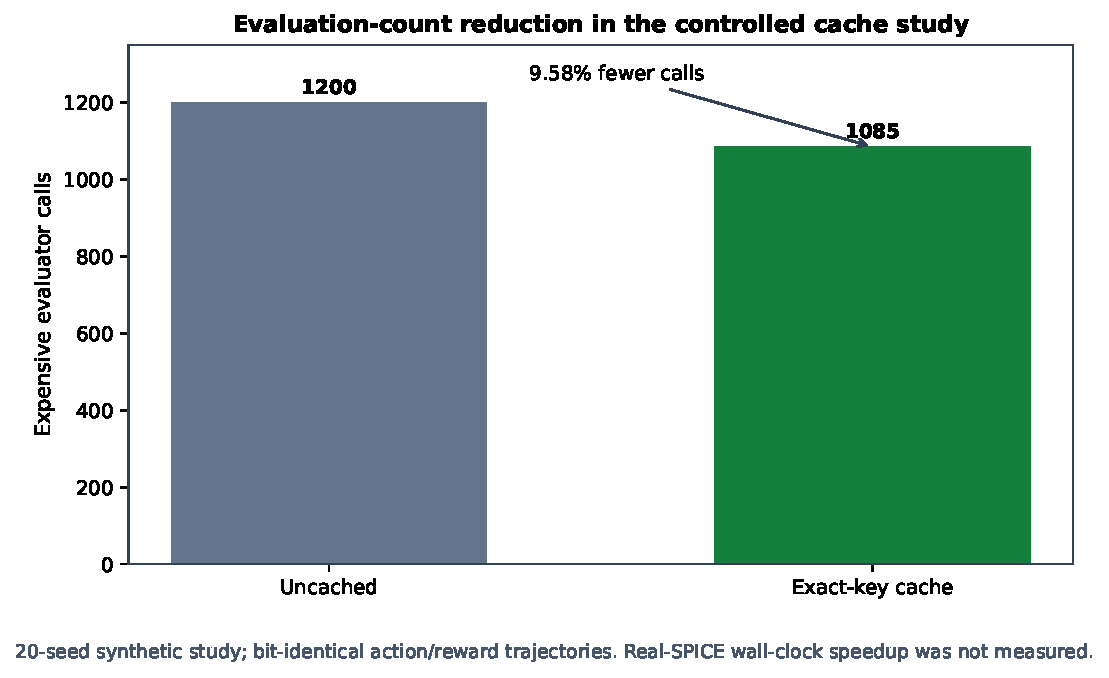
\includegraphics[width=0.82\textwidth]{evaluation-efficiency.pdf}
  \caption{Evaluator-call reduction from the controlled 20-seed synthetic cache
  study. Identical inputs produced bit-identical trajectories. The figure does
  not claim a measured real-SPICE wall-clock speedup.}
  \label{fig:cache-efficiency}
\end{figure}

\begin{landscape}
\begin{figure}[p]
  \centering
  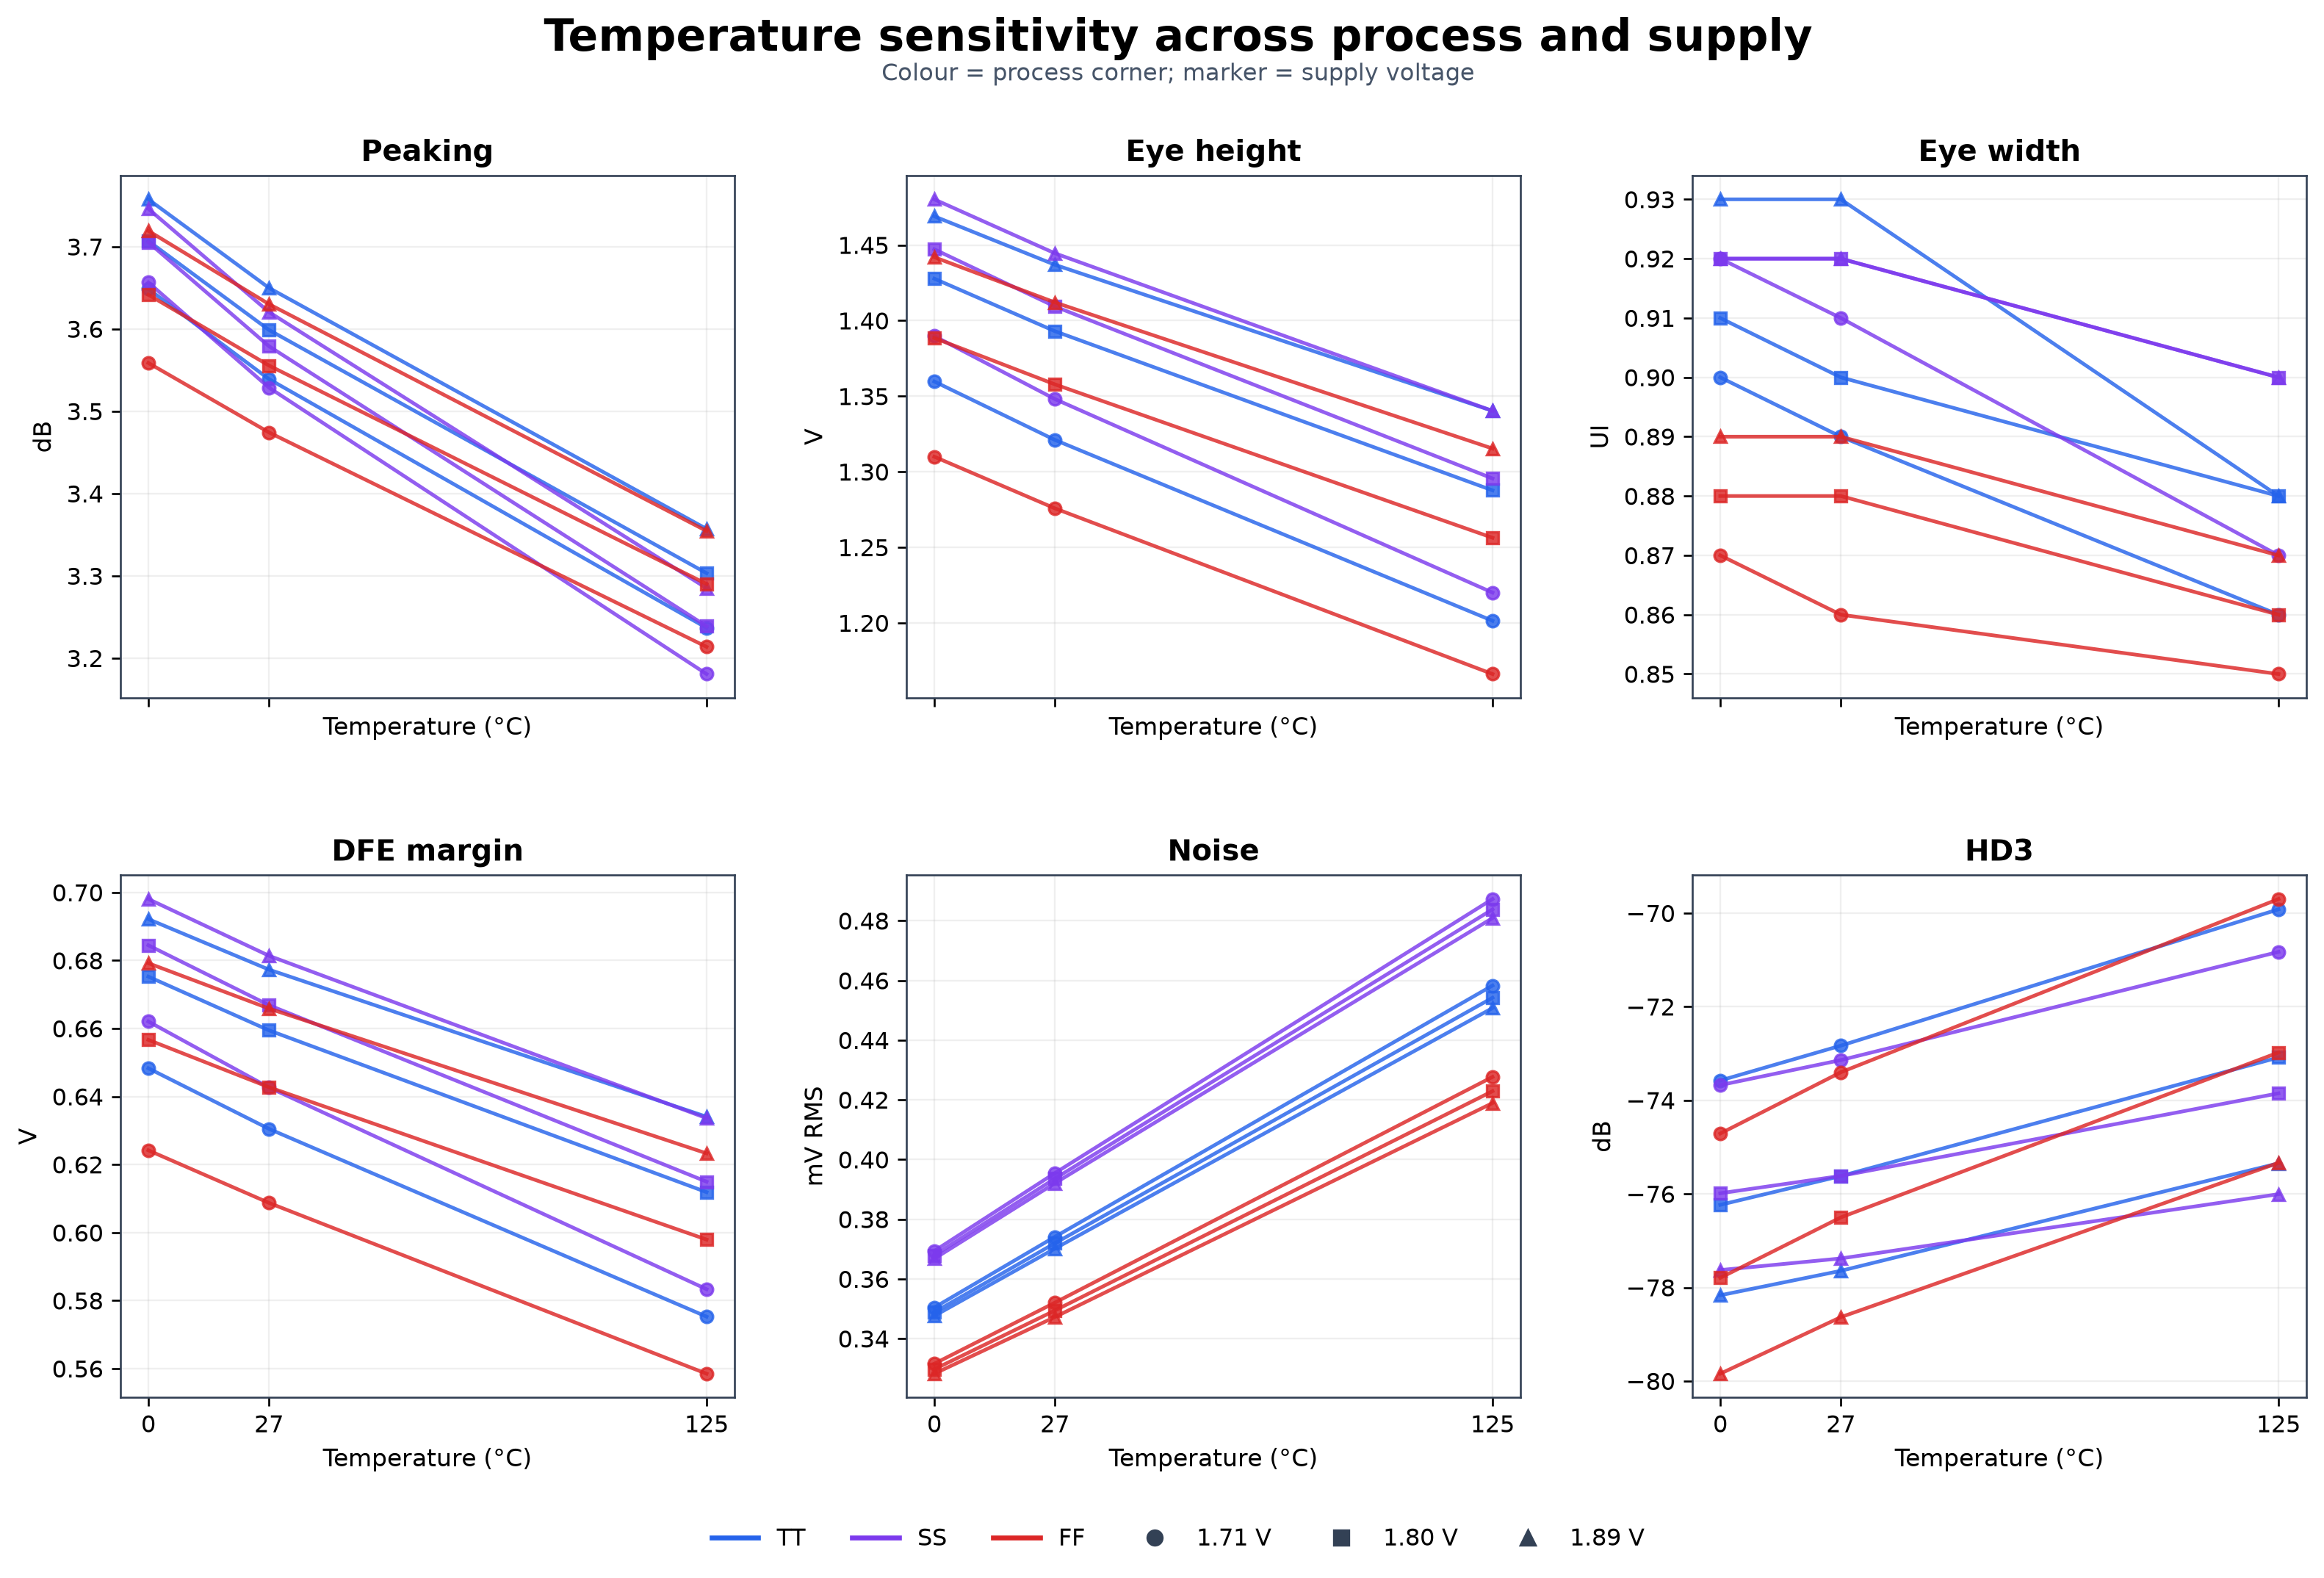
\includegraphics[width=0.95\linewidth]{pvt27-temperature-trends.png}
  \caption{Temperature trends across process and supply for the completed
  reduced 27-condition run. Color identifies process corner and marker shape
  identifies supply. Only 0, 27, and \SI{125}{\degreeCelsius} were evaluated.}
  \label{fig:pvt-temperature}
\end{figure}
\end{landscape}

\begin{figure}[p]
  \centering
  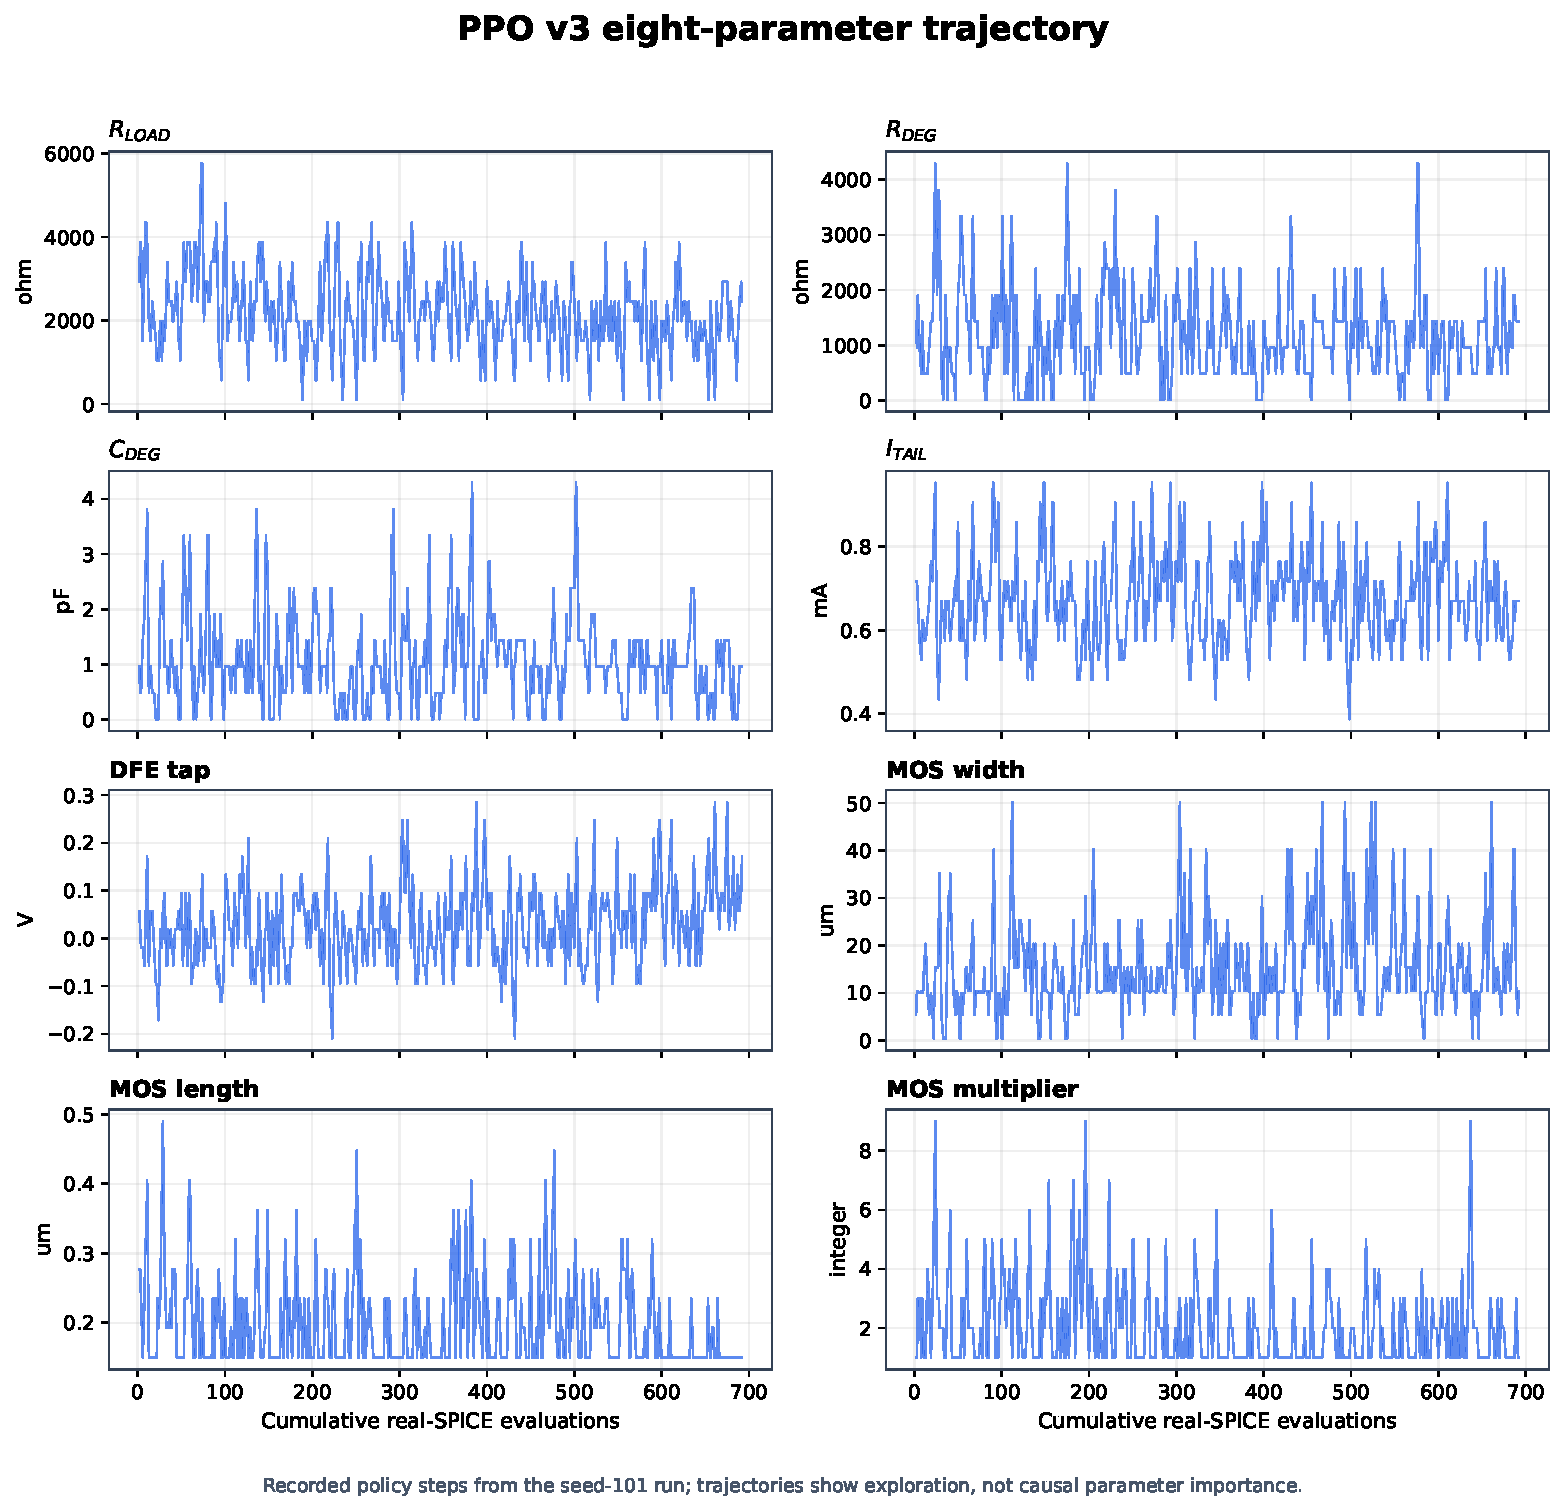
\includegraphics[width=0.96\textwidth,height=0.82\textheight,keepaspectratio]{ppo-v3-parameter-trajectory.pdf}
  \caption{Eight-parameter policy-step trajectory for the seed-101 v3 run. The
  traces show explored parameter values against cumulative evaluations; they do
  not establish causal parameter importance or convergence.}
  \label{fig:parameter-trajectory}
\end{figure}


\bibliographystyle{IEEEtranN}
\bibliography{references}

\end{document}
